\chapter{Reti di Petri}
\label{Capitolo 5}
% \begin{center}
%   \begin{tikzpicture}[node distance=2cm, bend angle=45, auto]

%     \node [transition] (t) [below right of = py, label=right:$"t"$] {};
%     \node [place] (p1) [above of = t, label=right:$$] {$p_1$};
%     \node [place] (p2) [below of = t, label=right:$$] {$p_2$};
%     \path[-{Latex[width=2mm]}]
%     (p1) edge (t)
%     (t) edge (p2)

%   \end{tikzpicture}
% \end{center}
Abbiamo introdotto un'algebra di processi come CCS dove processi sequenziali
interagiscono tra loro tramite handshaking. Un altro modello usato, con varie
implementazioni, sono gli automi a stati finiti (usati per reti neurali,
riconoscitori di linguaggi, modelli di protocolli di comunicazioni
etc$\ldots$).\\
Si passa ora alle \textbf{reti di Petri}, introdotte da \href{https://it.wikipedia.org/wiki/Carl_Adam_Petri}{Carl Adam Petri} nel 1962 nella sua
tesi di dottorato, partendo da una critica ai modelli fatti tramite automi a
stati per protocolli di comunicazioni.\\

La nuova teoria dei sistemi è basata sui principi della fisica quantistica, il
modello, nell’ottica di Petri, non è quindi un modello chiuso ma è 
in grado di \textbf{comunicare con l’ambiente} (in sintonia con le teorie della
fisica). Vuole una teoria dei sistemi in grado di descrivere il flusso di
informazioni e che permetta di analizzare sistemi con un'organizzazione
complessa.\\
La sua teoria generale dei sistemi che processano informazione si basa su, tra
le altre cose:
\begin{itemize}
  \item comunicazione
  \item sincronizzazione
  \item flusso di informazione
  \item relazione di concorrenza e indipendenza causale
\end{itemize}
A partire dagli anni '70 questa teoria si è sviluppata dal punto di vista
dell'espressività, portando allo studio di diverse classi di reti. Si sviluppano
anche tecniche formali di analisi e di verifica delle reti (tramite algebra
lineare, teoria dei grafi etc$\ldots$). Le reti di Petri hanno tantissimi ambiti
d'uso, tra i quali:
\begin{itemize}
  \item specificare protocolli di comunicazione
  \item disegnare circuiti asincroni
  \item algoritmi concorrenti/paralleli
  \item modellare sistemi organizzativi
  \item modellare db distribuiti
  \item specificare sistemi di controllo industriali
  \item modellare sistemi biologici e per modellare reazioni chimiche
  \item valutare le prestazioni (tramite reti stocastiche e temporizzate)
\end{itemize}
Il problema della rappresentazione dei sistemi concorrenti, mediante i sistemi di transizioni etichettati, è che lo stato globale non è
osservabile, inoltre la simulazione sequenziale non deterministica dei sistemi distribuiti è una
forzatura, non rispecchia il reale comportamento. Tali sistemi modellano un sistema con un insieme di stati e un insieme di transizioni, dove lo stato è globale, cioè uno stato è un elemento dell’insieme degli stati.
Come vedremo in seguito nelle reti di Petri gli stati sono locali e lo stato globale o caso, o configurazione, è dato dall’insieme di condizioni vere in quel determinato caso.
Allo stesso modo le transizioni o eventi sono transizioni locali, ovvero: la loro occorrenza dipende dalle loro pre-condizioni e post-condizioni e non dalla validità di condizioni (stati locali) che non hanno connessione con l’evento in oggetto.
Le reti di Petri (o sistemi elementari) presentano invece le seguenti caratteristiche:
\begin{itemize}
 \item Lo stato è definito da una collezione di stati locali ovvero le condizioni vere in quel momento 
 \item Gli eventi possono occorrere solamente se tutte le precondizioni dello stesso sono vere e tutte
le post condizioni sono false. Quando un evento occorre trasforma tutte le sue precondizioni
in false e le post in vere; questo meccanismo prende il nome di regola di scatto.
\item Gli eventi possono avvenire anche in maniera concorrente
\end{itemize}

  Una rete di Petri PT (Place/Transition) è un grafo orientato con due tipi di nodi, condizioni e eventi, connessi da archi diretti. I condizioni sono rappresentati graficamente da cerchi e le eventi da rettangoli.

Un arco può unire solamente nodi di tipo diverso, quindi possono esserci archi tra condizioni e eventi - ma non tra condizioni e condizioni o eventi e eventi. Una condizione da cui un arco parte per finire in un evento è detto condizione di input dell'evento; un condizione in cui un arco arriva partendo da una evento è detto condizione di output dell'evento.

I condizioni possono contenere un certo numero di token o marche. Una distribuzione di token sull'insieme dei condizioni della rete è detta marcatura. Gli eventi agiscono sui token in ingresso secondo una regola, detta regola di scatto (in inglese firing). Un evento è abilitata se può scattare, cioè se ci sono token in ogni condizione di input. Quando una evento scatta, essa consuma token dai suoi condizioni di input, esegue dei task e posiziona un numero specificato di token in ognuno dei suoi condizioni di uscita. Ciò avviene automaticamente, ad esempio in un singolo step non-prelazionabile. L'esecuzione delle reti di Petri è non deterministica. Ciò significa due cose:

    se più eventi sono abilitate nello stesso momento, una qualsiasi di esse può scattare ma
    non è garantito che una evento abilitato scatti; una evento abilitato può scattare immediatamente, dopo un tempo di attesa qualsiasi (a patto che resti abilitata), o non scattare affatto.

Poiché lo scatto di una evento non è predicibile a priori, le reti di Petri sono molto adatte a modellare il comportamento di un sistema concorrente. 


\section{Reti elementari}
Diamo una definizione generale degli argomenti che andremo a trattare.
Una rete descrive la struttura \textbf{statica} del sistema, il \textbf{comportamento} è invece definito da: 
\begin{itemize}
    \item \textbf{Regola si scatto}: un evento si dice abilitato quando tutte le sue precondizioni sono vere e tutte le
post sono false, se un evento si trova in questa situazione può scattare trasformando tutte le sue
precondizioni in false e le post-condizioni in vere. É rispettato il principio di estensionalità: quando
un evento scatta modifica solamente le sue pre e le sue post, le altre condizioni rimangono
inalterate.
    \item \textbf{Caso}: non è altro che un insieme di condizioni che rappresentano
l’insieme di condizioni vere in una certa configurazione del sistema.
\end{itemize}
Una rete che non ha auto anelli (per ogni evento, l’intersezione delle pre e delle post dello stesso è vuoto) si dice \textbf{pura}. Un insieme di eventi indipendenti è tale se per ogni evento nessuno ha pre o post condizioni in comune con un altro evento dell’insieme. Un passo è abilitato se due eventi possono scattare in maniera concorrente, questo può
succedere se i due eventi sono indipendenti.
Per introdurre i sistemi elementari delle reti di Petri, ovvero una classe molto
semplice e astratta, partiamo da un esempio:
\begin{esempio}
  Vediamo l'esempio del \textit{Produttore e del Consumatore}.\\
  Si ha un sistema con una componente Produttore che produce elementi e li
  deposita in un buffer che ha un'unica posizione (quindi o è pieno o è vuoto) e
  con un consumatore che preleva dal buffer un elemento per poi consumarlo ed
  essere pronto a prelevare un altro elemento. Si ha un comportamento
  ciclico. Usiamo quindi le reti di Petri, col modello dei sistemi elementari,
  per rappresentare questo modello. Bisogna quindi individuare le proprietà
  fondamentali locali del sistema.\\
  Partiamo dal produttore, che può avere 2 stati locali:
  \begin{enumerate}
    \item pronto per produrre
    \item pronto per depositare
  \end{enumerate}
  Usiamo i \textbf{cerchi} per rappresentare \textbf{condizioni locali} che sono
  associabili a delle proposizioni della logica che possono essere vere o
  false. Queste preposizioni sono quindi \textbf{stati locali}. Gli \textbf{eventi locali} vengono
  invece rappresentati con un \textbf{rettangolo}. Un evento ha un arco entrante
  da uno stato che rappresenta le \textit{precondizioni} di quell'evento (che
  devono essere vere per permettere l'occorrenza dell'evento). L'occorrenza
  dell'evento rende false le precondizioni e rende vere le
  \textit{post-condizioni} (che sono stati raggiungibili con un arco uscente da
  un evento). \textbf{Si ha quindi che il produttore può depositare solo se il buffer
  non è pieno, quindi le post-condizioni di un evento devono essere false
  affinché l'evento possa occorrere (oltre alle precondizioni vere).}\\
  Passiamo al consumatore che estrae solo se il buffer è pieno ed è pronto a
  prelevare. Si procede poi con la stessa logica del produttore di cambiamento
  tra vero e falso delle varie condizioni locali.\\
  In questo esempio si hanno quindi condizioni che sono preposizioni booleane e
  rappresentano stati locali. Si ha quindi a sinistra il produttore, a destra il
  consumatore e in mezzo il buffer:
  \begin{center}
    \begin{tikzpicture}[node distance=2cm, bend angle=45, auto]
      \node [place] (p0) [label=above:\small{pronto a depositare}] {};
      \node [transition] (t1) [below right of = p0, label=left:\small{deposita}] {};
      \node [transition] (t2) [below left of = p0, label=left:\small{produce}] {};
      \node [place] (p1) [below right of = t2, label=below:\small{pronto a produrre}]
      {}; 
      \node [place] (p3) [right of = t1, label=above:\small{buffer pieno}] {};
      \node [transition] (t4) [right of = p3, label=right:\small{estrae}] {};

      \node [place] (p2) [above right of = t4, label=above:\small{pronto a prelevare}]
      {}; 
      \node [transition] (t3) [below right of = p2, label=right:\small{consuma}] {};
      \node [place] (p4) [below right of = t4, label=below:\small{pronto a consumare}]
      {}; 
      
      \path[-{Latex[width=2mm]}]
      (p0) edge (t1)
      (t1) edge (p1)
      (p1) edge (t2)
      (t2) edge (p0)
      (t1) edge (p3)
      (p3) edge (t4)
      (t4) edge (p4)
      (p4) edge (t3)
      (t3) edge (p2)
      (p2) edge (t4)
      ;
    \end{tikzpicture}
  \end{center}

 \textbf{ Lo stato globale del sistema è dato da una
  collezione di stati locali.} Per segnare tali condizioni mettiamo un punto
  pieno dentro il cerchio e queste condizioni ``abilitano'' i vari eventi:
  \begin{center}
    \begin{tikzpicture}[node distance=2cm, bend angle=45, auto]
      \node [place] (p0) [label=above:\small{pronto a depositare}] {};
      \node [transition] (t1) [below right of = p0, label=left:\small{deposita}] {};
      \node [transition] (t2) [below left of = p0, label=left:\small{produce}] {};
      \node [place, tokens=1] (p1) [below right of = t2, label=below:pronto a
      produrre] {}; 
      \node [place] (p3) [right of = t1, label=above:\small{buffer pieno}] {};
      \node [transition] (t4) [right of = p3, label=right:\small{estrae}] {};

      \node [place, tokens=1] (p2) [above right of = t4, label=above:pronto a
      prelevare] {}; 
      \node [transition] (t3) [below right of = p2, label=right:\small{consuma}] {};
      \node [place] (p4) [below right of = t4, label=below: \small{pronto a consumare}]
      {}; 
      
      \path[-{Latex[width=2mm]}]
      (p0) edge (t1)
      (t1) edge (p1)
      (p1) edge (t2)
      (t2) edge (p0)
      (t1) edge (p3)
      (p3) edge (t4)
      (t4) edge (p4)
      (p4) edge (t3)
      (t3) edge (p2)
      (p2) edge (t4)
      ;
    \end{tikzpicture}
  \end{center}
  Si può arrivare a una \textit{configurazione} dove, per esempio, sia l'evento
  \textit{produce}, del produttore, che l'evento \textit{estrae}, del
  consumatore, sono abilitati. Si ha quindi che i due eventi possono occorrere
  in modo \textbf{concorrente} infatti i due eventi sono \textbf{indipendenti}
  in quanto condizionati da \textbf{precondizioni e post-condizioni completamente
    disgiunte}. 
    \begin{nota}
    Due eventi che occorrono in maniera concorrente lo possono fare in
  qualsiasi ordine, non si ha infatti una sequenza temporale specifica tra i
  due. 
  In questo sistema quindi siano solo stati locali ed eventi localizzati e non
  stati ed eventi globali. Un evento dipende solo dalle sue precondizioni e
  dalle sue post-condizioni. E, in generale, un evento ha senso solo se modifica delle condizioni. \textit{Se rappresentiamo con delle marche le condizioni vere possiamo
    simulare il comportamento del sistema con il \textit{gioco delle marche} che
    mostra come l'evoluzione delle condizioni avviene all'occorrenza degli
    eventi.}     \end{nota}

  La simulazione di un tale sistema può comunque avvenire con un sistema di
  transizioni etichettato, ovvero con un automa a stati finiti, che rappresenta
  gli stati globali corrispondenti alle diverse combinazioni di stati locali che
  di volta in volta sono veri.
  \newpage
  Gli archi vengono etichettati con gli eventi che
  comportano un cambiamento di stato globale:
 \begin{center}
    \begin{tikzpicture}[node distance=2cm, bend angle=45, auto]
      \node [place] (p0) [label=above:\small{P2}] {};
      \node [transition] (t1) [below right of = p0, label=left:\small{d}] {};
      \node [transition] (t2) [below left of = p0, label=left:\small{p}] {};
      \node [place, tokens=1] (p1) [below right of = t2, label=below:\small{P1}] {}; 
      \node [place] (p3) [right of = t1, label=above:\small{B}] {};
      \node [transition] (t4) [right of = p3, label=right:\small{e}] {};

      \node [place, tokens=1] (p2) [above right of = t4, label=above:\small{C1}] {}; 
      \node [transition] (t3) [below right of = p2, label=right:\small{c}] {};
      \node [place] (p4) [below right of = t4, label=below:\small{C2}]
      {}; 
      
      \path[-{Latex[width=2mm]}]
      (p0) edge (t1)
      (t1) edge (p1)
      (p1) edge (t2)
      (t2) edge (p0)
      (t1) edge (p3)
      (p3) edge (t4)
      (t4) edge (p4)
      (p4) edge (t3)
      (t3) edge (p2)
      (p2) edge (t4)
      ;
    \end{tikzpicture}
  \end{center}
  \begin{figure}[H]
    \centering
    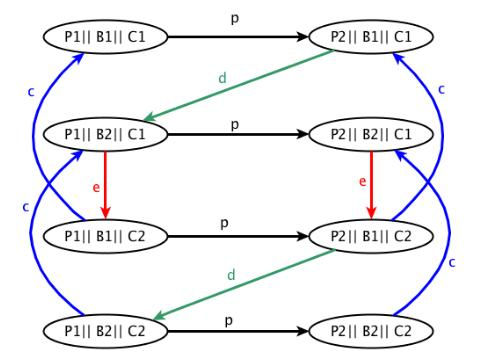
\includegraphics[scale = 0.6]{img/prod3.jpg}
    \caption{Rappresentazione del sistema con un automa a stati finiti che
      rappresenta stati globali}
  \end{figure}
  Lo stesso evento in algebra di processi sarebbe (espandendo il buffer $"B"$ in
  un modo che poi specificheremo per specificare pieno e vuoto):
  \[S=(P1|B1|C1)_{\{\backslash deposita, estae\}}\]
  \[P1=produce\cdot P2\]
  \[P2=\overline{deposita}\cdot P1\]
  \[C1=estrae\cdot C2\]
  \[C2=consuma\cdot C1\]
  \[B1=deposita\cdot B2\]
  \[B2=\overline{estae}\cdot B1\]
\end{esempio}
\subsection{Formalizzazione di una rete elementare}
Passiamo ora alla formalizzazione di questi aspetti.\\
\begin{definizione}
  Una \textbf{rete elementare} è definita come una tripla:
  \[N=(B, E, F)\]
  dove:
  \begin{itemize}
    \item $"B"$ è un insieme finito di \textbf{condizioni}, ovvero \textit{stati
      locali}, proprietà/proposizioni booleane etc$\ldots$. Vengono
    rappresentate con un cerchio 
    \item $"E"$ è un insieme finito di \textbf{eventi}, ovvero trasformazioni
    locali di stato e \textit{transizioni locali}. Vengono rappresentate con un
    quadrato o con un rettangolo pieno
    \item $"F"$ è una \textbf{relazione di flusso} che connette condizioni ad
    eventi ed eventi a condizioni. Si ha quindi che:
    \[F\subseteq (B\times E)\cup(E\times B)\]
    Le relazioni di flusso sono rappresentate da archi orientati. Inoltre la
    relazione di flusso è tale per cui non esistano \textbf{elementi isolati},
    in quanto non avrebbero senso, in un tale sistema, eventi isolati (che non
    modificherebbero mai una condizione) o condizioni isolate (che non
    verrebbero mai modificate da un evento). Si ha, formalmente, che: 
    \[dom(F)\cup ran(F)=B\cup E\]
    ovvero non abbiamo condizioni/eventi isolati, in quanto non avrebbero senso
    (potremmo anche non modellarle), avremmo una condizione costante e un
    evento che non accade mai, quindi dvigili del fuocoo e codvigili del fuocoo di $"F"$ coprono
    l'insieme di condizioni ed eventi
  \end{itemize}
  Si ha che:
  \[B\cap E = \emptyset\]
  \[B\cup E \neq \emptyset\]
  Ovvero gli insiemi delle condizioni e degli eventi sono tra loro disgiunti e
  non vuoti.\\
  \subsection{Pre e Post}
  \begin{definizione}
    
  Sia ora $"x"$ un elemento qualsiasi della rete, \textbf{ovvero $"x"$ può essere o una
  condizione o un evento}, formalmente:
  \[x\in B\cup E\]
  Si ha che, dato $X=B\cup E$:
  \begin{itemize}
    \item $^\bullet x=\{y\in X:\,(y, x)\in F\}$ rappresenta l'insieme di tutti gli
    elementi $"y"$ che sono connessi dalla relazione di flusso ad $"x"$, ovvero si
    ha un arco da $"y"$ a $"x"$. Sono quindi i \textbf{pre-elementi} di $"x"$, ovvero
    le \textit{precondizioni}, se $"x"$ è un evento, o i \textit{pre-eventi}, se
    $"x"$ è una condizione
    \item $x^\bullet=\{y\in X:\,(x, y)\in F\}$ rappresenta l'insieme di tutti gli
    elementi $"y"$ che sono connessi dalla relazione di flusso a partire da $"x"$,
    ovvero si ha un arco da $"x"$ a $"y"$. Sono quindi i \textbf{post-elementi} di
    $"x"$, ovvero le \textit{post-condizioni}, se $"x"$ è un evento, o i
    \textit{post-eventi}, se $"x"$ è una condizione
  \end{itemize}
  
  \end{definizione} \vspace{5mm} %5mm vertical space
  \begin{corollario}
     possiamo estendere questa notazione a insiemi di elementi. Sia $"A"$ un insieme
  qualsiasi di elementi, che possono quindi essere sia condizioni che eventi:
  \[A\subseteq B\cup E\]
  Si ha quindi che i pre-elementi dell'insieme $"A"$ sono rappresentati con:
  \[^\bullet A=\cup_{x\in A}\, ^\bullet x\]
  ovvero l'unione dei pre-elementi di ogni singolo elemento dell'insieme $"A"$.\\
  Analogamente si ha che i post-elementi dell'insieme $"A"$ sono rappresentati
  con: 
  \[A^\bullet=\cup_{x\in A} x^\bullet\]
  ovvero l'unione dei post-elementi di ogni singolo elemento dell'insieme $"A"$.
    \end{corollario}
  \begin{nota}
  Nelle reti c'è sempre una relazione di \textbf{dualità} tra due
    elementi, per esempio tra condizioni ed eventi, tra pre-eventi e
    post-eventi, tra pre-condizioni e post-condizioni. Inoltre si ha la
    caratteristica della \textbf{località}, quindi si hanno stati locali e
    trasformazioni di stato locali
  \end{nota}
\end{definizione} \vspace{5mm} %5mm vertical space
\subsection{Configurazione e evento}
La rete $N=(B, E, F)$ descrive la \textit{struttura statica del sistema}, il
comportamento è definito attraverso le nozioni di \textbf{caso (o
  configurazione)} e di \textbf{regola di scatto (o di evento)}.\\
\begin{definizione}
  Un \textbf{caso} (o \textbf{configurazione}) è un insieme di condizioni
  $c\subseteq B$ che rappresentano l’insieme di condizioni \textbf{vere} in una certa
  configurazione del sistema, un insieme di \textbf{stati locali} che
  collettivamente individuano lo \textbf{stato globale} del sistema.\\
  Graficamente le condizioni vere presentano un puntino in mezzo al cerchio
  mentre le condizioni false solo un cerchio vuoto:
  \begin{center}
    \begin{tikzpicture}[node distance=2cm, bend angle=45, auto]
      \node [place] (p0) [label=above:\small{False}] {};
      \node [place, tokens=1] (p1) [right of = p0, label=above:\small{True}] {};
      {}; 
      
    \end{tikzpicture}
  \end{center}
\end{definizione} \vspace{5mm} %5mm vertical space
\begin{definizione}
  Sia $N=(B, E, F)$ una rete elementare e sia $c\subseteq B$ una certa
  configurazione (non serve quindi necessariamente conoscere tutto lo stato del
  sistema). La \textbf{regola di scatto} mi permette di stabilire quando
  un evento $e\in E$ è abilitato, ovvero può occorrere in $"c"$:
  \[^\bullet e\subseteq c \,\,\,\,\land\,\,\,\, e^\bullet \cap c = \emptyset\]
  \textbf{ovvero sse tutte le precondizioni dell'evento sono vere (e quindi sono
  contenute nella configurazione $"c"$) e sse tutte le post-condizioni sono false
  (quindi non si hanno intersezioni tra le post-condizioni e la
  configurazione).} \\
\end{definizione} \vspace{5mm} %5mm vertical space
\begin{nota}
  
  L'occorrenza o l'\textbf{abilitazione} di $"e"$ in $"c"$ si denota con la dicitura:
  \[c[e >\]
  \end{nota}
\begin{definizione}
  Se un evento $"e"$ è abilitato in $"c"$, ovvero $c[e >$, si ha che quando $"e"$
  occorre in $"c"$ genera un nuovo caso $c'$ e si usa la notazione:
  \[c[e > c'\]
  Si ha quindi che $c'$ è così calcolabile:
  \[c'=(c-^\bullet e)\cup e^\bullet\]
  Ovvero togliendo da $"c"$ tutte le precondizioni dell'evento $"e"$ e aggiungendo
  quindi tutte le post-condizioni di $"e"$
\end{definizione} \vspace{5mm} %5mm vertical space
\begin{definizione}
  Le reti si basano sul \textbf{principio di estensionalità}, ovvero sul fatto che
il cambiamento di stato è locale:
\begin{center}
  \textit{Un evento è completamente caratterizzato dai cambiamenti che produce
    negli stati locali, tali cambiamenti sono indipendenti dalla particolare
    configurazione in cui l’evento occorre.}
\end{center}
Ovvero: quando
un evento scatta modifica solamente le sue pre e le sue post, le altre condizioni rimangono
inalterate.
\end{definizione} \vspace{5mm} %5mm vertical space
L'importante è che le precondizioni di un evento siano vere e le post-condizioni
false (siamo comunque interessati solo alla validità delle condizioni che
riguardano l'evento).
\begin{nota}
non importa il valore di verità delle condizioni che \textbf{non} toccano un evento
\end{nota}
\begin{esempio}
  Partendo da:
  \begin{center}
    \begin{tikzpicture}[node distance=2cm, bend angle=45, auto]
      \node [place] (p0) [label=above:\small{P2}] {};
      \node [transition] (t1) [below right of = p0, label=left:\small{d}] {};
      \node [transition] (t2) [below left of = p0, label=left:\small{p}] {};
      \node [place, tokens=1] (p1) [below right of = t2, label=below:\small{P1}] {}; 
      \node [place, tokens=1] (p3) [right of = t1, label=above:\small{B}] {};
      \node [transition] (t4) [right of = p3, label=right:\small{e}] {};

      \node [place, tokens=1] (p2) [above right of = t4, label=above:\small{C1}] {}; 
      \node [transition] (t3) [below right of = p2, label=right:\small{c}] {};
      \node [place] (p4) [below right of = t4, label=below:\small{C2}]
      {}; 
      
      \path[-{Latex[width=2mm]}]
      (p0) edge (t1)
      (t1) edge (p1)
      (p1) edge (t2)
      (t2) edge (p0)
      (t1) edge (p3)
      (p3) edge (t4)
      (t4) edge (p4)
      (p4) edge (t3)
      (t3) edge (p2)
      (p2) edge (t4)
      ;
    \end{tikzpicture}
  \end{center}
  \newpage
  Può scattare $"e"$ e portare a:
   \begin{center}
    \begin{tikzpicture}[node distance=2cm, bend angle=45, auto]
      \node [place] (p0) [label=above:\small{P2}] {};
      \node [transition] (t1) [below right of = p0, label=left:\small{d}] {};
      \node [transition] (t2) [below left of = p0, label=left:\small{p}] {};
      \node [place, tokens=1] (p1) [below right of = t2, label=below:\small{P1}] {}; 
      \node [place] (p3) [right of = t1, label=above:\small{B}] {};
      \node [transition] (t4) [right of = p3, label=right:\small{e}] {};

      \node [place] (p2) [above right of = t4, label=above:\small{C1}] {}; 
      \node [transition] (t3) [below right of = p2, label=right:\small{c}] {};
      \node [place, tokens=1] (p4) [below right of = t4, label=below:\small{C2}]
      {}; 
      
      \path[-{Latex[width=2mm]}]
      (p0) edge (t1)
      (t1) edge (p1)
      (p1) edge (t2)
      (t2) edge (p0)
      (t1) edge (p3)
      (p3) edge (t4)
      (t4) edge (p4)
      (p4) edge (t3)
      (t3) edge (p2)
      (p2) edge (t4)
      ;
    \end{tikzpicture}
  \end{center}
  Quindi dato $C=\{P1, B, C1\}$ abbiamo che, dopo lo scatto dell'evento $"e"$
  (possibile visto che tutte le post-condizioni di $"e"$ sono disabilitate):
  \[C[e>C'\]
  con $C'=\{P1, C2\}$.
  ($P1$ resta inalterato, per il \textbf{principio di estensionalità}).
\end{esempio}
\begin{definizione}
  Sia $N=(B, E, F)$ una rete elementare. Possiamo definire due tipologie di rete:
  \begin{enumerate}
    \item $"N"$ è definita \textbf{semplice} sse:
    \[\forall x, y \in B\cup E,\,\, (^\bullet x = ^\bullet y)\wedge (x^\bullet =
      y^\bullet)\Rightarrow x = y\]
    Ovvero per ogni coppia di elementi (che siano quindi eventi o condizioni) se
    i loro pre-elementi e i loro post-elementi coincidono allora non ha senso
    distinguere $"x"$ e $"y"$. Vediamo un esempio di rete non semplice, in quanto
    $P0$ e $P1$ rappresentano la stessa condizione e quindi non ha senso
    distinguerli: 
    \begin{center}
      \begin{tikzpicture}[node distance=2cm, bend angle=45, auto]
        \node [place] (p0) [label=above:\small{P0}] {};
        \node [place] (p1) [right of = p0, label=above:\small{P1}] {}; 
        \node [place] (p2) [right of = p1, label=above:\small{P2}] {};
        \node [transition] (t1) [below right of = p0] {};
        \node [transition] (t2) [below left of = p2] {};
        \node [place] (p3) [left of = t1, label=below:\small{P3}] {}; 
        \node [place] (p4) [right of = t2, label=below:\small{P4}] {};
        {}; 
        
        \path[-{Latex[width=2mm]}]
        (p0) edge (t1)
        (p0) edge (t2)
        (p1) edge (t1)
        (p1) edge (t2)
        (p2) edge (t2)
        (t1) edge (p3)
        (t2) edge (p4)
        ;
      \end{tikzpicture}
    \end{center}
    \newpage
    Vale anche per eventi. Vediamo un esempio dove non ha senso distinguere $T1$
    e $T2$:
    \begin{center}
      \begin{tikzpicture}[node distance=2cm, bend angle=45, auto]
        \node [place] (p0) [] {};
        \node [place] (p1) [right of = p0] {};
        \node [transition] (t0) [left of = p0, label=above:\small{T0}] {};
        \node [transition] (t1) [below of = p0, label=left:\small{T1}] {};
        \node [transition] (t2) [below of = p1, label=right:\small{T2}] {};
        \node [place] (p3) [below of = t1] {}; 
        {}; 
        
        \path[-{Latex[width=2mm]}]
        (t0) edge (p0)
        (p0) edge (t1)
        (p0) edge (t2)
        (p1) edge (t1)
        (p1) edge (t2)
        (t1) edge (p3)
        (t2) edge (p3)
        ;
      \end{tikzpicture}
    \end{center}
    \item $"N"$ è definita \textbf{pura} sse:
    \[\forall e \in E:\,\,^\bullet e \cap e^\bullet = \emptyset\]
    Ovvero se per ogni evento non esiste una pre-condizione che sia anche
    post-condizioni. Si ha quindi un \textbf{cappio} (detto anche \textbf{side
      condition}) tra un evento e una condizione. Avere questa situazione
    comporta che l'evento non può scattare in quanto la condizione che per lui è
    sia una pre-condizione che una post-condizioni non può essere
    contemporaneamente vera e falsa, l'evento non potrà mai scattare e quindi
    non potrà mai essere osservato. Non avrebbe quindi senso modellarlo. Vediamo
    un esempio:
    \begin{center}
    \begin{tikzpicture}[node distance=2cm, bend angle=45, auto]
      \node [place] (p0) [] {};
      \node [transition] (t1) [below right of = p0] {};
      \node [place] (p1) [right of = p0] {}; 
      \node [place] (p3) [right of = t1] {};


      {}; 
      
      \path[-{Latex[width=2mm]}]
      (p0) edge [bend left = 25](t1)
      (t1) edge [bend left = 25](p0)
      (p1) edge (t1)
      (t1) edge (p3)
      ;
    \end{tikzpicture}
  \end{center}
    
  \end{enumerate}
\end{definizione} \vspace{5mm} %5mm vertical space
\begin{nota}
In questo libro considereremo sempre \textbf{reti pure}.
\end{nota}
\subsection{Indipendenza tra eventi}
\begin{definizione}
  Data una rete elementare $N=(B, E, F)$ e sia $U \subseteq E$ un sottoinsieme di
  eventi e siano $c, c_1, c_2\in B$ tre configurazioni. Si ha che:
  \begin{itemize}
    \item $"U"$ è un \textbf{insieme di eventi indipendenti} sse:
    \[\forall e_1, e_2\in U:\,\, e_1\neq e_2\Rightarrow (^\bullet e_1\cup
      e_1^\bullet)\cap  (^\bullet e_2\cup e_2^\bullet) = \emptyset\]
    Ovvero se per ogni evento nessuno ha pre o post condizioni in
comune con un altro evento dell’insieme.
    \item $"U"$ è un \textbf{passo abilitato}, ovvero un insieme di \textit{eventi
      concorrenti} in una certa configurazione $"c"$, che si indica con:
    \[c[U>\]
    sse:
    \[U \mbox{ è un insieme di eventi indipendenti } \wedge\,\, \forall e\in
      U:\,\, c[e>\]
      Ciò implica che più eventi possono scattare in maniera concorrente, questo può
succedere se gli eventi dell'insieme sono indipendenti in una determinata configurazione, ovvero hanno pre-condizioni e post-condizioni differenti/disgiunte.
    \item $"U"$ è un \textbf{passo} dalla configurazione $c_1$ alla configurazione
    $c_2$, che si indica con:
    \[c_1[U > c_2\]
    sse:
    \[(c_1[U) \wedge \Big(c_2=(c_1-^\bullet U)\cup U^\bullet\Big)\]
    ovvero sse $"U"$ è un passo abilitato in $c_1$ e lo scatto degli eventi in $"U"$
    porta alla configurazione $c_2$ che si ottiene togliendo da $c_1$ l'insieme
    delle precondizioni degli eventi in $"U"$ e aggiungendo quindi l'insieme delle
    post-condizioni degli eventi in $"U"$.
  \end{itemize}
\end{definizione} \vspace{5mm} %5mm vertical space
\begin{esempio}
  Preso:
   \begin{center}
    \begin{tikzpicture}[node distance=2cm, bend angle=45, auto]
      \node [place] (p0) [label=above:\small{P2}] {};
      \node [transition] (t1) [below right of = p0, label=left:\small{d}] {};
      \node [transition] (t2) [below left of = p0, label=left:\small{p}] {};
      \node [place, tokens=1] (p1) [below right of = t2, label=below:\small{P1}] {}; 
      \node [place, tokens=1] (p3) [right of = t1, label=above:\small{B}] {};
      \node [transition] (t4) [right of = p3, label=right:\small{e}] {};

      \node [place, tokens=1] (p2) [above right of = t4, label=above:\small{C1}] {}; 
      \node [transition] (t3) [below right of = p2, label=right:\small{c}] {};
      \node [place] (p4) [below right of = t4, label=below:\small{C2}]
      {}; 
      
      \path[-{Latex[width=2mm]}]
      (p0) edge (t1)
      (t1) edge (p1)
      (p1) edge (t2)
      (t2) edge (p0)
      (t1) edge (p3)
      (p3) edge (t4)
      (t4) edge (p4)
      (p4) edge (t3)
      (t3) edge (p2)
      (p2) edge (t4)
      ;
    \end{tikzpicture}
  \end{center}
  si ha che:
  \begin{itemize}
    \item $\{p, e\},\{p, c\},\{d, c\}$ sono esempi di insiemi di eventi
    indipendenti
    \item $\{p, e\}$ è un passo abilitato in $\{P_1, B, C_1\}$
    \item $\{P_1, B, C_1\}[\{p, w\}>\{P_2, C_2\}$ è lo scatto del passo
    $\{p, e\}$.
  \end{itemize}
\end{esempio}
\section{Sistema Elementare}
Cominciamo a definire alcuni concetti che rivedremo più dettagliatamente nel corso della trattazione.\\
Un sistema elementare è definito da una rete (definizione vista sopra ’N’) e da un caso iniziale.\\
L’insieme dei casi raggiungibili può essere definito induttivamente come segue: il caso iniziale è
un caso raggiungibile e ogni caso raggiunto facendo un passo da un caso raggiungibile, è un
caso raggiungibile.\\
Il comportamento dei sistemi elementari può essere descritto in 3 modi:
\begin{itemize}
    \item Sequenza di occorrenze ed eventi: in questo modo si descrive il comportamento sequenziale
del sistema
    \item Sequenza di passi: in questo modo è possibile descrivere il comportamento non sequenziale
del sistema
    \item Processi non sequenziali: in questo metodo si cattura une registrazione di quello che ha fatto
un processo eseguendo il sistema. Viene descritto il comportamento non sequenziale.
\end{itemize}

Diamo ora una definizione formale di \textbf{sistema elementare}.
\begin{definizione}
  Un \textbf{sistema elementare} $\Sigma=(B, E, F;c_{in})$ è definito come una
  rete elementare $N=(B, E, F)$ e a cui è associato un caso iniziale, una configurazione
  iniziale, ovvero un sottoinsieme di condizioni che rappresentano lo stato
  iniziale da cui inizia la computazione e l'evoluzione del sistema. Formalmente
  il caso iniziale si indica con $C_{in}\in B$ 
\end{definizione} \vspace{5mm} %5mm vertical space
\subsubsection{Casi Raggiungibili}
\begin{definizione}
  Dato un sistema elementare $\Sigma=(B, E, F;c_{in})$ si indica con $C_\Sigma$
  l'insieme dei \textbf{casi raggiungibili} da tale sistema a partire dal caso
  iniziale $c_{in}$.\\
  Formalmente l'insieme dei casi raggiungibili è il di piccolo sottoinsieme
  dell'insieme delle parti di $"B"$, ovvero $2^B$, tale che:
  \begin{itemize}
    \item $c_{in}\in C_\Sigma$, ovvero sicuramente il caso iniziale appartiene
    all'insieme dei casi raggiungibili
    \item se $c\in C_\Sigma,\, U\subseteq E$ e $c'\subseteq B$ sono tali che
    $c[U>c'$ allora $c'\in C_\Sigma$, ovvero se abbiamo un generico caso $"c"$ che
    appartiene ai casi raggiungibili, se abbiamo un insieme di eventi $"U"$ tale che
    questo insieme di eventi (che abbiamo visto essere indipendenti, per la
    definizione di passo abilitato) è abilitato
    in $"c"$ in un unico passo e la sua occorrenza mi porta in $c'$, allora anche
    $c'$ appartiene a $C_\Sigma$. 
  \end{itemize}
 \begin{nota}
  Questa è una definizione data per \textbf{induzione strutturale}, nel primo
  punto si ha la base, nel secondo l'ipotesi e la conseguenza.
 \end{nota}
\end{definizione} \vspace{5mm} %5mm vertical space
\subsubsection{Insieme dei passi}
\begin{definizione}
  Dato un sistema elementare $\Sigma=(B, E, F;c_{in})$ si indica con $U_\Sigma$
  l'\textbf{insieme dei passi} di $\Sigma$, ovvero di tutti i possibili \textbf{insiemi}
  di eventi indipendenti che possono occorrere in qualche caso. Formalmente:
  \[U_\Sigma =\{U\subseteq E\,|\,\exists\, c, c'\in C_\Sigma :\, c[U>c'\}\]
  Ovvero l'insieme dei sottoinsiemi di eventi tali per cui esistano due casi
  raggiungibili in $C_\Sigma$ e $"U"$ è abilitato in $"c"$ e il suo scatto mi porta
  in $c'$.
\end{definizione} \vspace{5mm} %5mm vertical space
\subsection{Comportamento dei sistemi elementari}
\begin{definizione}
  Sia $\Sigma=(B, E, F;c_{in})$ un sistema elementare e siano $c_i\in C_\Sigma$ ed
  $e_i\in E$.\\
  Definiamo;
  \begin{itemize}
    \item un \textbf{comportamento sequenziale} come una sequenza di eventi che
    possono occorrere dal caso iniziale. Facendo scattare in maniera sequenziale
    gli eventi uno alla volta in $c_n$:
    \[c_{in} [e_1 > c_1 [e_2 > \ldots[e_n > c_n\]
    Scrittura che può essere alleggerita in:
    \[c_{in} [e_1 e_2 \ldots e_n > c_n\]
    Possiamo dire di avere a che fare con una \textbf{simulazione sequenziale
      non deterministica, detta anche \textit{semantica a interleaving}},
    infatti abbiamo più eventi abilitati da prendere uno alla volta
    \item un \textbf{comportamento non sequenziale}, in quanto possiamo anche
    considerare insiemi di eventi, ovvero passi. Considero quindi sequenze di
    passi, avendo a che fare con la \textbf{step semantics}. Non abbiamo quindi una
    simulazione sequenziale non deterministica in quanto dal caso iniziale
    faccio scattare un insieme di eventi, in maniera concorrente (e quindi senza
    ordine specificato), per poi far scattare un altro insieme di eventi fino ad
    arrivare a $c_n$: 
    \[c_{in} [U_1 > c_1 [U_2 > \ldots [U_n > c_n\]
    Scrittura che può essere alleggerita in:
    \[c_{in} [U_1 U_2 \ldots U_n > c_n\]
    Gli insiemi $U_i$ non sono insiemi massimali abilitati ma sottoinsiemi
    indipendenti e abilitati in $c_{in}$.\\
\item    possiamo avere anche un altro tipo di \textbf{comportamento non sequenziale},
    definito da Petri stesso, in una \textbf{semantica a ordini parziali} (si
    parla anche di \textbf{true concurrency}) in
    cui si definiscono processi non sequenziali. Il comportamento di tale
    sistema viene registrato in una rete di Petri. Questo argomento verrà trattato integralmente nei prossimi capitoli.
  \end{itemize}
  In ogni caso si considerano sia sequenze finite che infinite (con cicli) di
  eventi o passi. 
\end{definizione} \vspace{5mm} %5mm vertical space
\newpage
\begin{esempio}
  Dato il sistema elementare $\Sigma$:
  \begin{figure}[H]
    \centering
    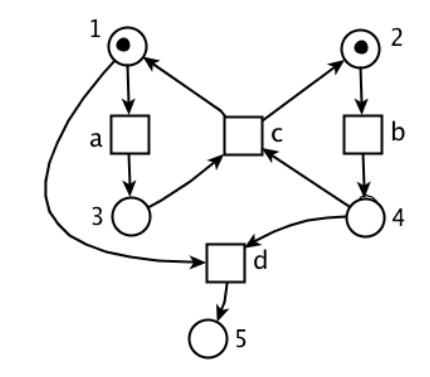
\includegraphics[scale = 0.4]{img/seq.jpg}
  \end{figure}
  si ha, per esempio, la seguente sequenza di occorrenza di eventi:
  \[\{1, 2\}[a > \{3, 2\}[b > \{3, 4\}[c > \{1, 2\}[b > \{1, 4\}[d > \{5\}\]
  arrivati in ``5'' abbiamo un caso finale, ovvero una situazione di
  \textbf{deadlock}, in quanto il sistema non può evolvere ulteriormente.\\
  Vediamo anche la seguente possibile sequenza di passi. In ``1'' e ``2'' sia
  ``a'' che ``b'' sono indipendenti e sono entrambi abilitati (scattano in
  maniera concorrente in un unico passo, ovviamente possiamo avere passi con lo
  scatto di un solo evento):
  \[\{1, 2\}[\{a, b\} > \{3, 4\}[\{c\} > \{1, 2\}[\{b\} > \{1, 4\}\]
  Come ricordato possiamo finire in una sequenza infinita.\\
  potremmo modellare un processo non sequenziale di $\Sigma$:
  \begin{figure}[H]
    \centering
    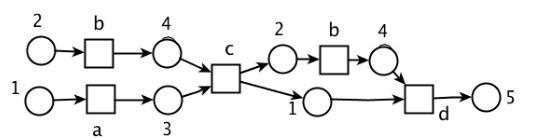
\includegraphics[scale = 0.4]{img/seq5.jpg}
  \end{figure}
\end{esempio}
\subsection{Modellare e registrare il comportamento di un sistema}
Il comportamento di un sistema elementare può essere rappresentato dal suo \textbf{grafo dei casi} (sequenziale o non sequenziale).
Questo grafo non è altro che un sistema di transizioni (LTS) etichettato dove le etichette sugli archi
rappresentano l’insieme di eventi che possono occorrere in un passo; questi archi collegano i vari
casi raggiungibili, formati da insiemi di condizioni vere.
\newpage
\subsubsection{Grafo dei casi raggiungibili}
\begin{definizione}
  Il \textbf{grafo dei casi raggiungibili} (o non sequenziale) di un sistema elementare
  $\Sigma=(B, E, F;c_{in})$ è il sistema di transizioni etichettato:
  \[CG_\Sigma=(C_\Sigma, U_\Sigma, A, c_{in})\]
  dove:
  \begin{itemize}
    \item $C_\Sigma$ è l'insieme dei nodi del grafo, ovvero gli stati globali,
    i casi raggiungibili dal sistema $\Sigma$    
    \item $U_\Sigma$, è l'alfabeto, ovvero i passi del sistema rappresentano
    l'alfabeto 
    \item $"A"$ è l'insieme di archi etichettati, formalmente definito come:
    \[A=\{(c, U, c')|\, c, c'\in C_\Sigma, U\in U_\Sigma, c[U>c'\}\]
    ovvero sono archi che connettono un caso $"c"$ con un caso $c'$ e sono
    etichettati con un passo $"U"$ sse $"U"$ è abilitato in $"c"$ e porta in
    $c'$. Ovviamente $"c"$ e $c'$ sono devono essere raggiungibili e $"U"$ deve
    appartenere all'insieme dei passi di $\Sigma$
  \end{itemize}
  Esempio in figura \ref{fig:gra}.
\end{definizione} \vspace{5mm} %5mm vertical space
\begin{figure}
  \centering
  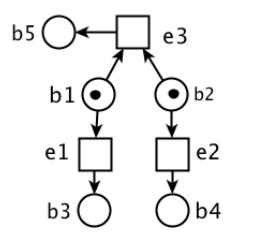
\includegraphics[scale = 0.5]{img/seq1.jpg}
  %\caption{Esempio di sistema $\Sigma$}
  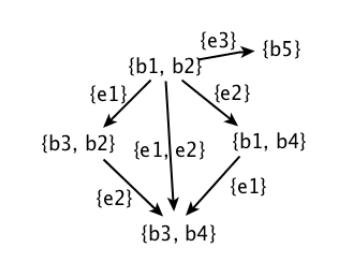
\includegraphics[scale = 0.5]{img/seq2.jpg}
  \caption{Esempio di sistema $\Sigma$ e il suo grafo dei casi del sistema
    $\Sigma$}
  \label{fig:gra}
\end{figure}
\subsubsection{Grafo dei casi sequenziale}
\begin{definizione}
  Un \textbf{grafo dei casi sequenziale} del sistema elementare
  $\Sigma=(B, E, F;c_{in})$ è una quadrupla:
  \[SCG_\Sigma=(C_\Sigma, E, A, c_{in})\]
  dove le etichette sono i singoli eventi (mentre il resto rimane definito come
  nel grafo dei casi raggiungibili). Formalmente si ha quindi che:
  \[A=\{(c, e, c')|\, c, c'\in C_\Sigma,\, e\in E:\, c[e>c'\}\]
  \begin{figure}[H]
    \centering
    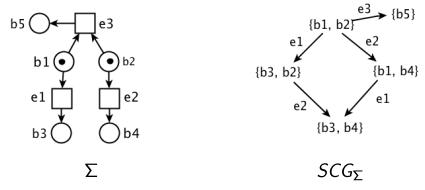
\includegraphics[scale = 0.6]{img/seq3.jpg}
    \caption{Esempio di grafo dei casi sequenziale}
  \end{figure}
  Si registra quindi l'occorrenza di un evento alla volta. Il grafo dei casi
  sequenziale è quindi il sistema di evento con gli archi etichettati dai
  singoli eventi.
  \begin{figure}[H]
    \centering
    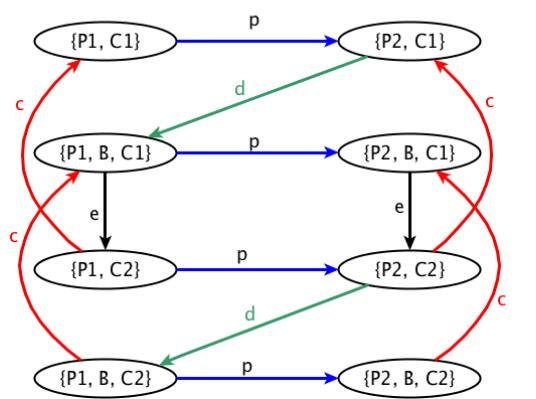
\includegraphics[scale = 0.4]{img/seqq.jpg}
    \caption{Esempio di grafo dei casi sequenziale dell'esempio con produttore
      e consumatore (con marche in $P1$ e $C1$)}
  \end{figure}
\end{definizione} \vspace{5mm} %5mm vertical space
\subsubsection{Diamond Property}
Grazie a questa proprietà possiamo dire che è sempre possibile ricavare dal grafo dei casi
sequenziale, il grafo dei casi non sequenziale/dei casi raggiungibili. In particolare  per passare da un grafo all'altro basta aggiungere le \textit{"diagonali"} in maniera esaustiva. 
 L'utilità di questa proprietà ricade nel concetto che potremmo anche non considerare il grafo dei casi
raggiungibili ma solo il \textbf{grafo dei casi sequenziale} (che è più comodo). Quindi se vale tale proprietà possiamo concludere che
questi due grafi sono quindi sintatticamente equivalenti.\\
La diamond property afferma che se si hanno due passi (insieme di eventi indipendenti abilitati in qualche caso)
disgiunti, e si ha un sottografo adatto, possiamo allora aggiungere la diagonale. In maniera più formale potremmo dire:
\begin{definizione}
  La \textbf{diamond property} stabilisce una proprietà della struttura del
  grafo della rete elementare, ovvero, dati $U_1, U_2\in U_\Sigma$ tali che:
  \begin{itemize}
    \item $U_1\cap U_2=\emptyset$
    \item $U_1\neq\emptyset$
    \item $U_2\neq\emptyset$
  \end{itemize}
  e dati $c_i\in C_\Sigma$ allora possiamo aggiungere le diagonali.
\end{definizione} \vspace{5mm} %5mm vertical space
\begin{esempio}
  \begin{figure}[H]
    \centering
    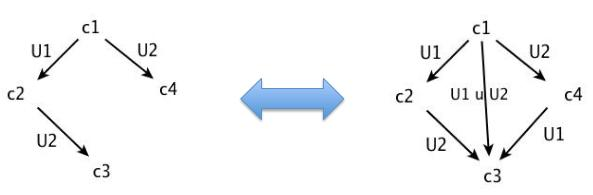
\includegraphics[scale = 0.6]{img/diam.jpg}
    \caption{Esempio di Diamond Property}
    \label{fig:dia}
  \end{figure}
Si possono fare delle prove:
\begin{enumerate}
  \item \textbf{prima prova:}\\
  Dimostriamo che possiamo passare all'immagine di destra da quella di sinistra
  aggiungendo i due archi mancanti, nella figura \ref{fig:dia}.\\
  Per semplicità diciamo che $U_i$ è un singolo evento $e_i$, con $i=1, 2$. Siano
  inoltre $c_1, c_2\in C_\Sigma$, ovvero sono casi raggiungibili, ed $e_1, e_2\in
  E$ tali che $c_1 [e_1 > c_2 [e_2 > \mbox{ e } c_1 [e_2 >$, i due eventi quindi
  sono abilitati in sequenza e da $c_1$ è anche abilitato $c_2$ . Si vuole
  dimostrare che: 
  \[(^\bullet e_1\cup e_1^\bullet)\cap(^\bullet e_2\cup e_2^\bullet)=\emptyset\]
  ovvero che i due eventi sono indipendenti, che sono entrambi abilitati e che
  sono eseguibili in qualsiasi ordine.
  \newpage
  Da $c_1 [e_1 > \mbox{ e }c_1 [e_2 >$ segue che:
  \begin{itemize}
    \item $^\bullet e_1\cap e_2^\bullet=\emptyset$
    \item $^\bullet e_2\cap e_1^\bullet=\emptyset$
  \end{itemize}
  infatti se $e_1$ e $e_2$ sono entrambi abilitati in $c_1$, le loro
  pre-condizioni sono vere e le post-condizioni false, e quindi non è possibile
  che una condizione sia contemporaneamente pre-condizione di $e_1$ (vera) e
  anche post-condizione di $e_2$ (falsa), e viceversa. Quindi le precondizioni
  di un evento sono disgiunte dalle post-condizioni dell'altro.\\
  Inoltre dal fatto che abbiamo $c_1 [e_1 > c_2 [e_2$, ovvero che da $c_1$ è
  abilitato $e_1$ e che dopo lo scatto di $e_1$ è ancora abilitato $e_2$
  possiamo dire che:
  \begin{itemize}
    \item $e_1^\bullet\cap e_2^\bullet=\emptyset$
    \item $^\bullet e_1\cap\, ^\bullet e_2=\emptyset$
  \end{itemize}
  in $c_2$, infatti, le pre-condizioni di $e_1$ sono false mentre le
  precondizioni di $e_2$ sono vere e quindi $e_1$ e $e_2$ non possono avere
  precondizioni in comune; inoltre sempre in $c_2$ le post-condizioni di $e_1$
  sono vere, mentre quelle di $e_2$ sono false, e quindi $e_1$ e $e_2$ non
  possono avere post-condizioni in comune. Quindi le precondizioni dei due
  eventi sono disgiunte, come del resto anche le post-condizioni, in quanto i due
  eventi sono sequenziali.\\
  Si è quindi dimostrato che i due eventi hanno precondizioni e post-condizioni
  completamente disgiunte e quindi la tesi è verificata
  \item \textbf{seconda prova:}\\
  Analizzando la situazione:
  \begin{figure}[H]
    \centering
    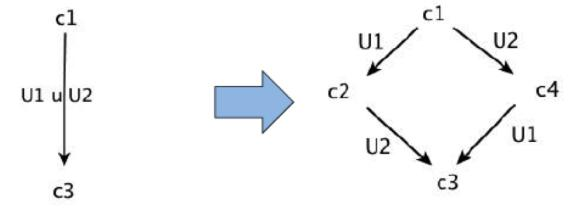
\includegraphics[scale = 0.45]{img/diam2.jpg}
  \end{figure}
  \newpage
  Si supponga che $U_1\cup U_2\in U_\Sigma$ e che si abbiano:
  \begin{itemize}
    \item $U_1\cap U_2=\emptyset$, ovvero sono disgiunti
    \item $U_1\neq\emptyset$
    \item $U_2\neq\emptyset$
  \end{itemize}
  allora se $c_1[(U_1\cup U_2)>c_3$, quindi è abilitato il passo $U_1\cup U_2$
  in $c_1$, sicuramente si ha che sono abilitati anche i singoli passi:
  \begin{itemize}
    \item $c_1[U_1>$
    \item $c_1[U_2>$
  \end{itemize}
  resta da dimostrare che dopo lo scatto di $U_1$ è ancora abilitato $U_2$ in
  $c_2$. Ma se $U_1\cup U_2$ è un passo abilitato significa che possiamo eseguirli
  in qualsiasi ordine, quindi anche prima $U_1$ e poi $U_2$, e questo comporta
  sicuramente che $U_2$ è abilitato e che porta a $c_3$. Analogamente invertendo
  $U_1$ e $U_2$, formalmente: 
  \begin{itemize}
    \item $c_1[U_1>c_2[U_2>c_3$
    \item $c_1[U_2>c_4[U_1>c_3$
  \end{itemize}
  Si dimostra così che l'immagine di sinistra comporta quella di destra.
\end{enumerate}
\end{esempio}
\begin{nota}
Riprendendo l'immagine precedente si ha che per la diamond property possono
aggiungere l'arco ``centrale'' che trasformerebbe nuovamente il grafo dei casi
sequenziale in quello dei casi raggiungibili quindi:
per la diamond property, nei sistemi elementari il grafo dei casi e il
  grafo dei casi sequenziale sono \textbf{sintatticamente equivalenti}, ovvero
  possono essere ricavati a vicenda e nessuno dei due fornisce più informazioni rispetto all'altro.
\end{nota}
  \begin{definizione}
    Dal \textbf{grafo sequenziale} si può ricostruire il \textbf{grafo dei casi} sse il sistema è elementare.
  \end{definizione} \vspace{5mm} %5mm vertical space

\subsection{Isomorfismo tra Sistemi di eventi Etichettati}
Si parla di isomorfismo quando due strutture complesse si possono
    applicare l'una sull'altra, cioè far corrispondere l'una all'altra, in modo
    tale che per ogni parte di una delle strutture ci sia una parte
    corrispondente nell'altra struttura; in questo contesto diciamo che due
    parti sono corrispondenti se hanno un ruolo simile nelle rispettive
    strutture.\\
Diamo ora una definizione formale di isomorfismo tra sistemi di evento
etichettati, che possono quindi essere grafi dei casi o grafi dei casi
sequenziali.
\begin{definizione}
  Siano dati due sistemi di evento etichettati:\\
  $A_1 = (S_1, E_1, T_1, s_{01})$ e $A_2 = (S_2 , E_2 , T_2 , s_{02})$.\\
  e siano date due \textbf{mappe biunivoche}:
  \begin{enumerate}
    \item $\alpha:S_1\to S_2$, ovvero che passa dagli stati del primo sistema a
    quelli del secondo
    \item $\beta:E_1\to E_2$, ovvero che passa dagli eventi del primo sistema a
    quelli del secondo
  \end{enumerate}
  allora:
  \[\langle \alpha,\beta\rangle:A_1= (S_1 , E_1 , T_1 , s_{01})\to A_2 = (S_2 ,
    E_2 , T_2 , s_{02})\]
  è un \textbf{isomorfismo} sse:
  \begin{itemize}
    \item $\alpha(s_{01})=s_{02}$, ovvero l'immagine dello stato iniziale del
    primo sistema coincide con lo stato iniziale del secondo
    \item $\forall s, s'\in S_1,\forall e\in E_1:\,(s, e, s')\in T_1
    \Leftrightarrow (\alpha(s),\beta(e),\alpha(s'))\in T_2$ ovvero per ogni
    coppia di stati del primo sistema, tra cui esiste un arco etichettato $"e"$,
    vale che esiste un arco, etichettato con l'immagine di $"e"$, nel secondo
    sistema che va dall'immagine del primo stato considerato del primo sistema
    all'immagine del secondo stato considerato del secondo sistema, e viceversa
  \end{itemize}
\end{definizione} \vspace{5mm} %5mm vertical space
\begin{definizione}
  Si definiscono \textbf{equivalenti} due \textbf{sistemi elementari} sse hanno grafi dei casi
  sequenziali, e quindi di conseguenza anche grafi dei casi (per la diamond property), \emph{isomorfi}.\\
  Due sistemi equivalenti accettano ed eseguono le stesse sequenze di eventi
\end{definizione} \vspace{5mm} %5mm vertical space
\subsection{Il Problema della Sintesi}
Si presenta ora un problema tipico dell'informatica, il \textbf{problema della
  sintesi}, ovvero dato un comportamento, o meglio una sua specifica, decidere
se esiste un'implementazione di tale specifica, ovvero un modello, che abbia
esattamente quel comportamento. Ovvero dato un sistema di transizioni etichettato stabilire se esiste un sistema
elementare tale che il suo grafo dei casi sia isomorfo al sistema di transizioni etichettato di
partenza. Questo problema è stato dimostrato essere risolvibile.
In questo caso dato un sistema di transizioni etichettato $A=(S, E, T, s_0)$, con:
\begin{itemize}
  \item $"S"$ insieme degli stati
  \item $"E"$ insieme delle etichette, ovvero degli eventi
  \item $"T"$ insieme delle transizioni
  \item $s_0$ stato iniziale
\end{itemize}

ci si propone di stabilire se esiste un sistema elementare
$\Sigma=(B, E, F;c_{in})$, tale che l'insieme degli eventi del sistema esattamente
l'insieme delle etichette di $"A"$ e tale che il suo grafo dei casi $SCG_\Sigma$
sia isomorfo ad $"A"$. Ci si propone anche di costruirlo.\\
Il problema è stato risolto mediante la cosiddetta \textbf{teoria delle regioni}
(che però non verrà trattato nel corso). Una \textbf{regione} comunque è un
  particolare sottoinsiemi di stati, legati tramite una certa condizione. Si può
  però dire che $"A"$ dovrà 
soddisfare la diamond property, in quanto altrimenti non sarebbe un sistema di
transizioni che potrebbe corrispondere al comportamento di un sistema
elementare.
\subsection{Contatti}
Cominciamo ad introdurre l'argomento in maniera poco formale: il contatto in una rete avviene quando un evento ha tutte le precondizioni vere ma non tutte le post
condizioni false. Un sistema privo da contatti è tale se ogni volta che le pre-condizioni sono vere,
necessariamente le post condizioni sono false. É possibile trasformare ogni rete in una priva di
contatti aggiungendo ad ogni evento il suo complemento. In un sistema privo di contatti è
sufficiente verificare che le precondizioni siano vere per essere sicuro che un evento può scattare.
\begin{definizione}
  Sia $\Sigma = (B, E, F;c_{in})$ un sistema elementare e siano $e\in E$ un evento
  e $c\in C_\Sigma$ un caso raggiungibile dal caso iniziale. Allora si ha che
  $(e, c)$ è un \textbf{contatto} sse:
  \[^\bullet e\subseteq c \wedge e^\bullet \cap c \neq\emptyset\]
  Ovvero, in termini pratici, siamo nel caso in cui un evento $"e"$ ha le
  precondizioni vere, si ha quindi che $^\bullet e\subseteq c$, e l'evento non
  ha tutte le post-condizioni false, quindi $e^\bullet \cap c \neq\emptyset$,
  allora si dice che l'evento $"e"$ è in una situazione di contatto e quindi non
  può scattare
  \begin{figure}[H]
    \centering
    \begin{tikzpicture}[node distance=2cm, bend angle=45, auto]
      \node [place, tokens=1] (p0) [label=above:\small{P2}] {};
      \node [transition] (t1) [below right of = p0, label=left:\small{d}] {};
      \node [transition] (t2) [below left of = p0, label=left:\small{p}] {};
      \node [place] (p1) [below right of = t2, label=below:\small{P1}] {}; 
      \node [place, tokens=1] (p3) [right of = t1, label=above:\small{B}] {};
      \node [transition] (t4) [right of = p3, label=right:\small{e}] {};

      \node [place, tokens=1] (p2) [above right of = t4, label=above:\small{C1}] {}; 
      \node [transition] (t3) [below right of = p2, label=right:\small{c}] {};
      \node [place] (p4) [below right of = t4, label=below:\small{C2}]
      {}; 
      
      \path[-{Latex[width=2mm]}]
      (p0) edge (t1)
      (t1) edge (p1)
      (p1) edge (t2)
      (t2) edge (p0)
      (t1) edge (p3)
      (p3) edge (t4)
      (t4) edge (p4)
      (p4) edge (t3)
      (t3) edge (p2)
      (p2) edge (t4)
      ;
    \end{tikzpicture}
    \caption{Esempio dove l'evento $"d"$ è in una situazione di
      contatto}
  \end{figure}
\end{definizione} \vspace{5mm} %5mm vertical space
\begin{definizione}
  Sia $\Sigma = (B, E, F;c_{in})$ un sistema elementare. Si dice che il sistema è
  \textbf{senza contatti} sse:
  \[\forall e\in E,\,\forall c\in C_\Sigma\mbox{ si ha che } ^\bullet
    e\subseteq c\Rightarrow e^\bullet\cap c=\emptyset\]
  ovvero per ogni evento e per ogni caso raggiungibile dal caso iniziale succede
  sempre che se le precondizioni sono vere, ovvero $^\bullet e\subseteq c$,
  allora le post-condizioni sono false, ovvero disgiunte dal caso considerato
  ($e^\bullet\cap c=\emptyset$)
\end{definizione} \vspace{5mm} %5mm vertical space
Ci si chiede se sia possibile trasformare un sistema elementare $\Sigma$, con
contatti, in uno $\Sigma'$, senza contatti, senza però modificarne il
comportamento.\\
La risposta a questo quesito è affermativa e la procedura consiste
nell'aggiungere a $\Sigma$ il complemento di ogni condizione che crea situazione
di contatto, ottenendo così un sistema $\Sigma'$ con grafo dei casi isomorfo a
quello di $\Sigma$.\\ 
Per aggiungere il complemento, data la condizione $"x"$, si aggiunge la condizione
$not\,\, x$ che sarà vera tutte le volte che $"x"$ è falsa e viceversa. Per
ottenere questo risultato la nuova condizione avrà come pre-eventi i
post-eventi di $"x"$ e come post-eventi i pre-eventi di $"x"$. Ovvero
connetto la nuova condizione agli stessi eventi di quella vecchia ma con archi
orientati in senso opposto. Ovviamente le inizializzazioni delle due condizioni
dovranno essere opposte (una vera e l'altra falsa).
\begin{figure}[H]
  \centering
  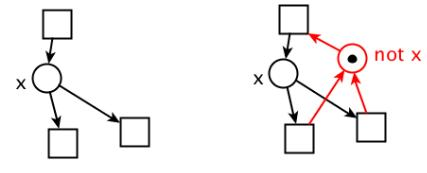
\includegraphics[scale = 0.6]{img/con2.jpg}
  \caption{Esempio con l'ottenimento del complemento di un sistema}
\end{figure}
Se un sistema è senza contatti si ha una regola di contatto semplificata:
\begin{definizione}
  Sia $\Sigma = (B, E, F;c_{in})$ un sistema elementare \textbf{senza
    contatti}. Sapendo che se le precondizioni di un evento sono vere allora
  sicuramente le post-condizioni di quell'evento sono false in quel caso. Dato
  che questo avviene per ogni evento e per ogni caso raggiungibile dal caso
  iniziale per verificare che un evento $"e"$ sia abilitato in un caso
  raggiungibile $"c"$ è sufficiente verificare che le precondizioni di $"e"$ siano
  vere (in quanto automaticamente le post-condizioni saranno false). In
  maniera formale quindi si ha che: 
  \[c[e\mbox{ sse } ^\bullet e\subseteq c,\,\,\mbox{ con } e\in E, c\in
    C_\Sigma\]
  semplificando di molto la \textbf{regola di scatto}:
\end{definizione} \vspace{5mm} %5mm vertical space
\begin{figure}[H]
  \centering
  \begin{tikzpicture}[node distance=2cm, bend angle=45, auto]
      \node [place, tokens=1] (p0) [label=above:\small{P2}] {};
      \node [transition] (t1) [below right of = p0, label=left:\small{d}] {};
      \node [transition] (t2) [below left of = p0, label=left:\small{p}] {};
      \node [place] (p1) [below right of = t2, label=below:\small{P1}] {}; 
      \node [place, tokens=1] (p31) [above right  of = t1, label=above:\small{B1}] {};
      \node [place] (p32) [ below right of = t1, label=below:\small{B2}] {};
      \node [transition] (t4) [below right of = p31, label=right:\small{e}] {};

      \node [place, tokens=1] (p2) [above right of = t4, label=above:\small{C1}] {}; 
      \node [transition] (t3) [below right of = p2, label=right:\small{c}] {};
      \node [place] (p4) [below right of = t4, label=below:\small{C2}]
      {}; 
      
      \path[-{Latex[width=2mm]}]
      (p0) edge (t1)
      (t1) edge (p1)
      (p1) edge (t2)
      (t2) edge (p0)
      (t1) edge (p32)
      (p32) edge (t4)
      (t4) edge (p31)
      (p31) edge (t1)
      
      (t4) edge (p4)
      (p4) edge (t3)
      (t3) edge (p2)
      (p2) edge (t4)
      ;
    \end{tikzpicture}
  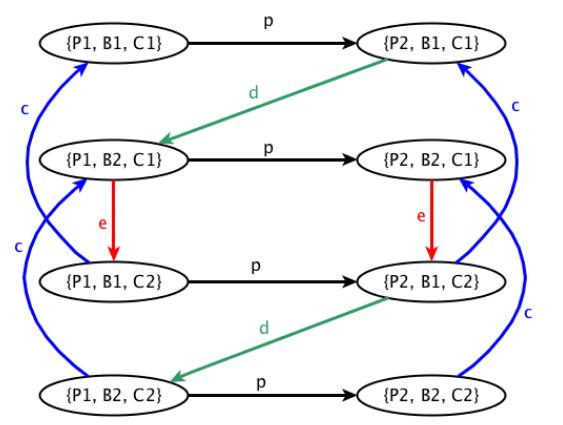
\includegraphics[scale = 0.4]{img/con33.jpg}
  \caption{Esempio con il complemento del sistema produttore-consumatore (dove è
    stato aggiunto solo il complemento di ``buffer-pieno'', ottenendo così sia
    $B1$ che $B2$, in quanto le altre condizioni avevano già il loro
    complemento). In aggiunta si ha anche il grafo dei casi sequenziale
    corrispondente al nuovo sistema senza contatti (grafo che è isomorfo a
    quello ottenibile al sistema con contatti)}
  \label{fig:con}
\end{figure}
\subsection{Situazioni Fondamentali}
\subsubsection{Sequenza}
Dato un sistema elementare, due eventi sono in sequenza se uno dipende
causalmente dall’altro. In parole piu semplici, se l’avvenire di un evento è subordinato
all’avvenire di un altro evento.
\begin{definizione}
  Sia $\Sigma = (B, E, F;c_{in})$ un sistema elementare, con contatti o meno
  e siano $c\in C_\Sigma$ un caso raggiungibile dal caso iniziale ed $e_1, e_2\in
  E$ due eventi.\\
  Si ha che $e_1$ ed $e_2$ sono \textbf{in sequenza} nel caso
  raggiungibile $"c"$ sse:
  \[c[e_1>\wedge\, \neg c[e_2\wedge c[e_1e_2>\]
  ovvero in $"c"$ è abilitato $e_1$ ma non $e_2$ ma, dopo lo scatto di $e_1$,
  $e_2$ diventa abilitato. Quindi in $"c"$ è possibile attivare prima $e_1$ e poi
  $e_2$ in sequenza.\\
  Si ha quindi una relazione di \textbf{dipendenza causale tra $e_1$ ed $e_2$},
  ovvero qualche post-condizione di $e_1$ è pre-condizione di $e_2$ (che quindi
  può occorrere solo se precedentemente è occorso $e_1$).
  \begin{figure}[H]
    \centering
    \begin{tikzpicture}[node distance=2cm, bend angle=45, auto]
      \node [place, tokens=1] (p0)  {};
      \node [transition] (t1) [right of = p0, label=above:$e_1$] {};
      \node [place] (p1) [above right  of = t1] {};
      \node [place] (p2) [right of = t1] {};
      \node [transition] (t2) [right  of = p1, label=above:$e_2$] {};
      \node [place] (p3) [right  of = t2] {};
      {}; 
      
      \path[-{Latex[width=2mm]}]
      (p0) edge (t1)
      (t1) edge (p1)
      (t1) edge (p2)
      (p1) edge (t2)
      (t2) edge (p3)
      ;
    \end{tikzpicture}
    \caption{Esempio di sequenza tra $e_1$ ed $e_2$}
  \end{figure}
\end{definizione} \vspace{5mm} %5mm vertical space
\subsubsection{Concorrenza}
Dato un caso raggiungibile e due eventi indipendenti (senza pre o post
condizioni in comune), i due eventi possono evolvere/scattare in un unico passo. In parole piu
semplici posso dire che se due eventi sono entrambi abilitati nello stesso istante, sono
concorrenti.
\begin{definizione}
  Sia $\Sigma = (B, E, F;c_{in})$ un sistema elementare, con contatti o meno
  e siano $c\in C_\Sigma$ un caso raggiungibile dal caso iniziale e $e_1, e_2\in
  E$ due eventi. \\
  Si ha che i due eventi sono \textbf{concorrenti} nel caso
  raggiungibile $"c"$ sse:
  \[c[\{e_1, e_2\}>\]
  ovvero se possono essere abilitati in unico passo o, detto in maniera
  diversa, se sono indipendenti ed entrambi abilitati in $"c"$
  \begin{figure}[H]
    \centering
    \begin{tikzpicture}[node distance=2cm, bend angle=45, auto]
      \node [place, tokens=1] (p0)  {};
      \node [place, tokens=1] (p00) [below of = p0] {};
      \node [transition] (t1) [right of = p0, label=above:$e_1$] {};
      \node [transition] (t2) [right of = p00, label=above:$e_2$] {};
      \node [place] (p1) [right  of = t1] {};
      \node [place] (p2) [right of = t2] {};
      \node [transition] (t3) [right of = p1] {};
      \node [place] (p3) [right of = t3] {};
      {}; 
      
      \path[-{Latex[width=2mm]}]
      (p0) edge (t1)
      (t1) edge (p1)
      (p1) edge (t3)
      (p00) edge (t2)
      (t2) edge (p2)
      (p2) edge (t3)
      (t3) edge (p3)
      ;
    \end{tikzpicture}
    \caption{Esempio di concorrenza tra $e_1$ ed $e_2$}
  \end{figure}
\end{definizione} \vspace{5mm} %5mm vertical space
\subsubsection{Conflitto}
Due eventi sono in conflitto se sono entrambi abilitati ma l’occorrenza di uno
disabilita l’altro. Intuitivamente possiamo dire che avviene quando due eventi condividono una
precondizione oppure un post condizione.
\begin{definizione}
  Sia $\Sigma = (B, E, F;c_{in})$ un sistema elementare, con contatti o meno
  e siano $c\in C_\Sigma$ un caso raggiungibile dal caso iniziale e $e_1, e_2\in
  E$ due eventi.\\
  Si ha che $e_1$ ed $e_2$ sono in conflitto sse:
  \[c[e_1>\,\wedge\, c[e_2 \wedge\,\neg c[\{e_1, e_2\}>\]
  ovvero i due eventi sono entrambi abilitati (quindi le precondizioni sono vere
  mentre le post-condizioni son false e gli eventi \textbf{non} sono indipendenti poiché hanno pre o post in comune) ma l'occorrenza di uno disabilità
  l'altro, quindi non possono essere abilitati in un unico passo, in quanto non
  sono indipendenti. Ci sono due casi:
  \begin{enumerate}
    \item i due eventi hanno una pre-condizione in comune, e in tal caso si parla
    di \textbf{conflitto forward} (ovvero \textit{in avanti})
    \begin{figure}[H]
      \centering
      \begin{tikzpicture}[node distance=2cm, bend angle=45, auto]
        \node [place, tokens = 1] (p0)  {};
        \node [transitionv] (t1) [above right of = p0, label=above:$e_1$] {};
        \node [transitionv] (t2) [below right of = p0, label=below:$e_2$] {};
        \node [place] (p1) [right  of = t1] {};
        \node [place] (p2) [right of = t2] {};
        {}; 
        
        \path[-{Latex[width=2mm]}]
        (p0) edge (t1)
        (t1) edge (p1)
        (p0) edge (t2)
        (t2) edge (p2)

        ;
      \end{tikzpicture}
      \caption{Esempio di conflitto forward tra $e_1$ ed $e_2$}
    \end{figure}
    \item i due eventi hanno una post-condizione in comune, e in tal caso si parla
    di \textbf{conflitto backward} (ovvero \textit{all'indietro})
    \begin{figure}[H]
      \centering
      \begin{tikzpicture}[node distance=2cm, bend angle=45, auto]
        \node [place, tokens = 1] (p0)  {};
        \node [place, tokens = 1] (p00) [below of = p0] {};
        \node [transitionv] (t1) [right of = p0, label=above:$e_1$] {};
        \node [transitionv] (t2) [right of = p00, label=below:$e_2$] {};
        \node [place] (p1) [right  of = t1] {};
        {}; 
        
        \path[-{Latex[width=2mm]}]
        (p0) edge (t1)
        (t1) edge (p1)
        (p00) edge (t2)
        (t2) edge (p1)
        ;
      \end{tikzpicture}
      \caption{Esempio di conflitto backward tra $e_1$ ed $e_2$}
    \end{figure}
  \end{enumerate}
  Si ha quindi una situazione di \textbf{non determinismo}, non essendo
  specificato quale dei due eventi scatterà prima (e lo scatto di uno impedisce
  lo scatto dell'altro).
  Possiamo ritrovarci nel caso in cui effettivamente un evento scatta, cambiando lo
  stato del sistema. In tal caso, in un'ottica completamente deterministica, si
  deve assumere che \textbf{l'ambiente} abbia fornito un'informazione
  riguardo il conflitto, ovvero c'è stato qualcosa di esterno che ha permesso ad
  uno dei due eventi di scattare ugualmente. abbiamo quindi guadagnato
  dell'informazione. 
  \begin{figure}[H]
    \centering
    \begin{tikzpicture}[node distance=2cm, bend angle=45, auto]
      \node [place] (p0)  {};
      \node [transitionv] (t1) [above right of = p0, label=above:$e_1$] {};
      \node [transitionv] (t2) [below right of = p0, label=below:$e_2$] {};
      \node [place, tokens=1] (p1) [right  of = t1] {};
      \node [place] (p2) [right of = t2] {};
      {}; 
      
      \path[-{Latex[width=2mm]}]
      (p0) edge (t1)
      (t1) edge (p1)
      (p0) edge (t2)
      (t2) edge (p2)

      ;
    \end{tikzpicture}
    \caption{Esempio di conflitto con l'intervento dell'ambiente tra $e_1$ ed
      $e_2$ (con conseguente guadagno di informazione)} 
  \end{figure}
  Ci sono però casi in cui in ogni caso non si può avere informazione su quale
  esempio sia scattato. Si può ipotizzare che tale informazione fosse presente
  nello stato precedente del sistema (una sola condizione attiva, per
  esempio). Quindi l'informazione, finita nell'ambiente (ricevuta
  dall'ambiente), si è persa.
  \begin{figure}[H]
    \centering
    \begin{tikzpicture}[node distance=2cm, bend angle=45, auto]
        \node [place] (p0)  {};
        \node [place] (p00) [below of = p0] {};
        \node [transitionv] (t1) [right of = p0, label=above:$e_1$] {};
        \node [transitionv] (t2) [right of = p00, label=below:$e_2$] {};
        \node [place, tokens = 1] (p1) [right  of = t1] {};
        {}; 
        
        \path[-{Latex[width=2mm]}]
        (p0) edge (t1)
        (t1) edge (p1)
        (p00) edge (t2)
        (t2) edge (p1)
        ;
      \end{tikzpicture}
    \caption{Esempio di conflitto tra $e_1$ ed
      $e_2$ con conseguente perdita di informazione (si può ipotizzare, per
      esempio, che nello stato precedente la pre-condizione di $e_1$ fosse attiva
      mentre quella dio $e_2$ fosse inattiva)} 
  \end{figure}
  Il modello, nell'ottica di Petri, non è quindi un \textbf{modello chiuso} ma è
  in grado di comunicare con l'ambiente (in sintonia con le teorie della
  fisica). 
\end{definizione} \vspace{5mm} %5mm vertical space
\subsubsection{Confusione}
Quando non è possibile stabilire oggettivamente un conflitto ci si trova in
situazione di confusione. Chi ha deciso? Chi ha la responsabilità di decidere?
\begin{definizione}
  La situazione di \textbf{confusione} è una \textit{mistura} di situazioni di
  concorrenza e di conflitto. Si hanno 2 tipi di confusione, entrambe
  ammissibili: 
  \begin{enumerate}
    \item detta \textbf{confusione asimmetrica} considera il fatto di avere un
    caso raggiungibile e due eventi abilitati, nella figura $e_1$ ed $e_2$, in
    maniera concorrente in $"c"$, che nella figura consiste nel caso
    $\{b_1, b_2, b_3\}$. I due eventi sono quindi indipendenti. Nella figura lo
    scatto dei due eventi porterebbe allo stato $c'=\{b_4, b_5\}$. Bisogna
    analizzare però nel dettaglio il sistema. Se prima occorre $e_1$ non si ha
    alcun conflitto mentre se occorre prima $e_2$ (che porterebbe in
    $\{b_1, b_3, b_4\}$) si crea un conflitto tra $e_1$ ed $e_3$, che viene
    risolto a favore di $e_1$ e a sfavore di $e_3$. \textbf{Non è possibile
      stabilire oggettivamente se è stato sciolto un conflitto}. Sono quindi in
    una situazione di confusione in quanto non so se è stata effettuata o meno
    una scelta.
    \begin{figure}[H]
      \centering
      \begin{tikzpicture}[node distance=2cm, bend angle=45, auto]
        %\node [place, tokens = 1] (p0)  {};
        \node [transition] (t1) [ label=right:$e_2$] {};
        \node [place, tokens = 1] (p0) [left of = t1,  label=left:$b_2$] {};
        \node [place] (p1) [below  of = t1,  label=left:$b_4$] {};
        \node [place, tokens = 1] (p2) [left  of = p1, label=left:$b_3$] {};
        \node [place, tokens = 1] (p3) [left  of = p2,  label=left:$b_1$] {};
        \node [transition] (t2) [below of = p1, label=left:$e_3$] {};
        \node [transition] (t3) [below of = p3, label=right:$e_1$] {};
        \node [place] (p4) [below of = t2, label=left:$b_6$] {};;
        \node [place] (p5) [below of = t3,  label=left:$b_5$] {};
        {}; 
        
        \path[-{Latex[width=2mm]}]
        (p0) edge (t1)
        (t1) edge (p1)
        (p1) edge (t2)
        (p2) edge (t2)
        (p2) edge (t3)
        (p3) edge (t3)
        (t2) edge (p4)
        (t3) edge (p5)
        ;
      \end{tikzpicture}
      \caption{Esempio di confusione asimmetrica tra $e_1$ ed $e_2$} 
    \end{figure}

    \item \textbf{Confusione simmetrica}, nome dovuto al fatto che la rete
    risulta disegnata in modo simmetrico, comportando delle
    problematiche. Prendiamo nell'immagine il caso raggiungibile $c=\{b_1, b_2\}$
    e i due eventi $e_1$ ed $e_3$, abilitati in maniera concorrente. Si ha che
    $c[\{e_1, e_3\}>c'$, con $c'=\{b_3, b_5\}$. Anche in questo caso si hanno dei
    conflitti, infatti sia $e_1$ che $e_3$ sono in conflitto con $e_2$ (in
    quanto se uno dei due viene eseguito $e_2$ non può più occorrere). Anche in
    questo caso non possiamo stabilire se il conflitto è stato risolto nel momento
    in cui arrivo in $c'$ (ovvero se si è deciso di fare $e_1$ piuttosto che
    $e_2$ o $e_3$ piuttosto che $e_2$).\\
    Anche in questo caso potremo dividere in componenti (una che esegue $e_1$ ed
    $e_2$ e un'altra che esegue $e_1$ ed $e_3$, con $e_2$ che è una
    sincronizzazione tra le due componenti).\\
    Non si può dire chi ha deciso e chi ha la responsabilità di decidere quale
    evento deve occorrere, se alla componente di $b_1$ o a quella di $b_2$.\\
    \begin{figure}[H]
      \centering
      \begin{tikzpicture}[node distance=2cm, bend angle=45, auto]
        \node [place, tokens = 1] (p0) [label=left:$b_1$] {};
        %\node [place, tokens = 1] (p1) [right of = p0, label=left:$b_2$] {};
        \node [transition] (t1) [below left of = p0, label=right:$e_1$] {};
        \node [transition] (t2) [below right of = p0, label=right:$e_2$] {};
        \node [place, tokens = 1] (p1) [above right of=t2, label=left:$b_2$] {};
        \node [transition] (t3) [below right of = p1, label=right:$e_3$] {};
        \node [place] (p3) [below of = t1, label=left:$b_3$] {};;
        \node [place] (p4) [below of = t2,  label=left:$b_4$] {};
        \node [place] (p5) [below of = t3,  label=left:$b_5$] {};
        {}; 
        
        \path[-{Latex[width=2mm]}]
        (p0) edge (t1)
        (p0) edge (t2)
        (p1) edge (t2)
        (p1) edge (t3)
        (t1) edge (p3)
        (t2) edge (p4)
        (t3) edge (p5)
        ;
      \end{tikzpicture}
      \caption{Esempio di confusione simmetrica tra $e_1$ ed $e_2$} 
    \end{figure}
  \end{enumerate}
  Petri era convinto, nella sua visione deterministica e senza conflitti, che
  l'avere una situazione di confusione nel modello fosse dovuto al non aver
  esplicitato alcuni aspetti o di aver costruito male il modello, con
  informazioni parziali e non complete sul modello e sull'ambiente.\\
  Un altro studioso, Einar Smith, molto vicino a Petri ha invece dimostrato come
  la confusione sia inevitabile
\end{definizione} \vspace{5mm} %5mm vertical space
Vediamo un esempio famoso, detto della \textbf{mutua esclusione}, portato da
Smith per spiegare come la confusione sia inevitabile nella realtà.
\newpage
\begin{esempio}
  Si analizza il seguente sistema:
  \begin{figure}[H]
    \centering
    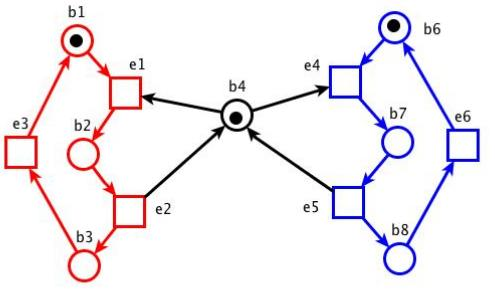
\includegraphics[scale = 0.4]{img/mes.jpg} 
  \end{figure}
  In rosso e in Blu abbiamo specificate le due componenti del sistema, che
  condividono una risorsa, ovvero la condizione $b_4$, che rappresenta che la
  risorsa è libera e a disposizione. L'evento $e_1$ e l'evento $e_4$ rappresentano
  eventi di acquisizione della risorsa (rispettivamente per la prima e per la
  seconda componente) e quindi le loro precondizioni rappresentano la necessità
  di acquisirla. Tra questi due eventi c'è una \textbf{situazione di
    conflitto}. Le condizioni $b_2$ e $b_7$, ovvero le rispettive post-condizioni
  dei due eventi, rappresentano che la risorsa è in uso per la rispettiva
  componente mentre gli eventi $e_2$ ed $e_5$ rappresentano il rilascio della
  risorsa condivisa, sempre per la rispettiva componente, arrivando
  rispettivamente nella componente $b_3$ e $b_8$. Ovviamente la risorsa
  non può essere contemporaneamente in uso da entrambe le risorse, quindi $b_2$
  e $b_7$ non possono essere contemporaneamente marcate, ovvero vere, e per
  questo si parla di \textit{mutua esclusione} (se una delle due è vera l'altra
  deve essere necessariamente falsa). D'altro canto gli
  eventi $e_3$ ed $e_6$ possono invece occorrere in modo concorrente senza
  conflitti.\\
  Scrivendo formalmente si ha che, nel caso che la risorsa sia stata acquisita
  dalla componente rossa e successivamente rilasciata:
  \[\{b_3, b_4, b_6\}[\{e_3, e_4\}>\{b_1, b_7\}\]
  \textbf{ma se scatta prima $e_3$ abbiamo il conflitto tra $e_1$ ed $e_4$, se scatta prima
  $e_4$ non abbiamo conflitti con $e_1$. Quindi non abbiamo informazioni sulla risoluzione
  del conflitto.}\\
\end{esempio}
\section{Sottoreti}
Partiamo subito con una definizione formale:
\begin{definizione}
  Siano $N=(B, E, F)$ e $N_1=(B_1, E_1, F_1)$ due reti elementari.\\
  Si dice che $N_1$ è \textbf{sottorete} di $"N"$ sse:
  \begin{itemize}
    \item $B_1\subseteq B$, quindi l'insieme delle condizioni della rete $N_1$
    è sottoinsieme di quello della rete $"N"$
    \item $E_1\subseteq E$, quindi l'insieme degli eventi della rete $N_1$
    è sottoinsieme di quello della rete $"N"$
    \item $F_1=F\cap[(B_1\times E_1)\cup (E_1\times B_1)]$, ovvero la relazione
    di flusso di $N_1$ è definita come la restrizione della relazione di flusso
    di $"N"$ rispetto alle condizioni e $B_1$ e agli eventi $E_1$ (tengo quindi
    solo gli archi di $"N"$ che connettono eventi e condizioni di $N_1$)
  \end{itemize}
\end{definizione} \vspace{5mm} %5mm vertical space
\begin{definizione}
  Siano $N=(B, E, F)$ e $N_1=(B_1, E_1, F_1)$ due reti elementari.\\
  Si dice che $N_1$ è \textbf{sottorete generata da} $B_1$ di $"N"$ (ovvero di
  sottorete generata da un insieme di condizioni) sse:
  \begin{itemize}
    \item $B_1\subseteq B$, quindi l'insieme delle condizioni della rete $N_1$
    è sottoinsieme di quello della rete $"N"$
    \item $E_1=\, ^\bullet B_1\cup B_1^\bullet$, ovvero come eventi si
    hanno tutti quegli eventi che sono collegati in $"N"$ alle condizioni incluse
    nell'insieme di condizioni $B_1$, prendendo quindi tutti i pre-eventi e i
    post-eventi delle condizioni dell'insieme $B_1$
    \item $F_1=F\cap[(B_1\times E_1)\cup (E_1\times B_1)]$, ovvero la relazione
    di flusso di $N_1$ è definita come la restrizione della relazione di flusso
    di $"N"$ rispetto alle condizioni $B_1$ e agli eventi $E_1$
  \end{itemize}
  Non abbiamo quindi una sottorete generata da un insieme arbitrario di condizioni ed
  eventi ma questi ultimi sono direttamente presi in relazione all'insieme delle
  condizioni scelto
\end{definizione} \vspace{5mm} %5mm vertical space
\begin{definizione}
  Siano $N=(B, E, F)$ e $N_1=(B_1, E_1, F_1)$ due reti elementari.\\
  Si dice che $N_1$ è \textbf{sottorete generata da} $E_1$ di $"N"$ (ovvero di
  sottorete generata da un insieme di eventi) sse:
  \begin{itemize}
    \item $B_1=\,^\bullet E_1\cup E_1^\bullet$, ovvero come condizioni si
    hanno tutte quelle condizioni che sono collegati in $"N"$ agli eventi inclusi
    nell'insieme di eventi $E_1$, prendendo quindi tutte e precondizioni e le
    post-condizioni degli eventi dell'insieme $E_1$
    \item $E_1\subseteq E$, quindi l'insieme degli eventi della rete $N_1$
    è sottoinsieme di quello della rete $"N"$
    \item $F_1=F\cap[(B_1\times E_1)\cup (E_1\times B_1)]$, ovvero la relazione
    di flusso di $N_1$ è definita come la restrizione della relazione di flusso
    di $"N"$ rispetto alle condizioni $B_1$ e agli eventi $E_1$
  \end{itemize}
  Non abbiamo quindi una sottorete generata da un insieme arbitrario di condizioni ed
  eventi ma le prime sono direttamente prese in relazione all'insieme degli
  eventi scelto
\end{definizione} \vspace{5mm} %5mm vertical space
\begin{esempio}
  Tornando all'esempio della mutua esclusione:
  \begin{figure}[H]
    \centering
    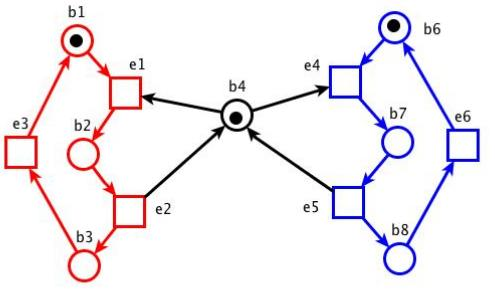
\includegraphics[scale = 0.4]{img/mes.jpg} 
  \end{figure}
  si ha, per esempio:
  \begin{itemize}
    \item in rosso si ha la sottorete $N'=(\{b_1, b_2, b_3\},
    \{e_1, e_2, e_3\}, F')$, che è la sottorete generata  dall'insieme di
    condizioni $B'=\{b_1, b_2, b_3\}$ 
    \item in blu si ha la sottorete $N'=(\{b_6, b_7, b_8\},
    \{e_4, e_5, e_6\}, F')$, che è la sottorete generata dall'insieme di condizioni
    $B'=\{b_6, b_7, b_8\}$
    \item si ha la sottorete $N'=(\{b_2, b_4, b_7\},\{e_1, e_2, e_4, e_5\}, F')$, che
    è la sottorete generata  dall'insieme di condizioni $B'=\{b_2, b_4, b_7\}$
    \item si ha la sottorete $N'=(\{b_1, b_2, b_3, b_4\},\{e_1, e_2, e_3\}, F')$, che
    è la sottorete generata da  dall'insieme di eventi $E'=\{e_1, e_2, e_3\}$
  \end{itemize}
\end{esempio}
\subsection{Operazioni di Composizione per Reti di Petri}
Data una rete $N=(B, E, F, c_0)$ questa può essere ottenuta componendo altre reti
di Petri. Si hanno in letteratura 3 modi principali:
\begin{enumerate}
  \item la \textbf{composizione sincrona}
  \item la \textbf{composizione asincrona}
  \item la \textbf{composizione mista, tra sincrona e asincrona}
\end{enumerate}
\newpage
Iniziamo informalmente a vedere degli esempi pratici.
\begin{esempio}
  Supponiamo di avere i modelli di due componenti, $N_1$, con un evento che
  corrisponde ad un'azione di invio, ed $N_2$, con un evento che corrisponde ad
  un'azione di ricezione:
  \begin{figure}[H]
    \centering
    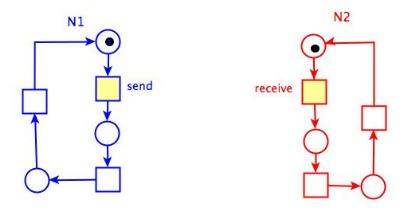
\includegraphics[scale = 0.5]{img/sinc.jpg} 
  \end{figure}
  Supponiamo che invio e ricezione siano eventi corrispondenti all'handshacking,
  ovvero l'invio avviene solo se può avvenire la ricezione.\\
  Vado quindi a sincronizzare questi due eventi, che diventano quindi un'unico
  evento nella rete composta, che è abilitato se le due precondizioni, nelle due
  componenti sono entrambe vere: 
  \begin{figure}[H]
    \centering
    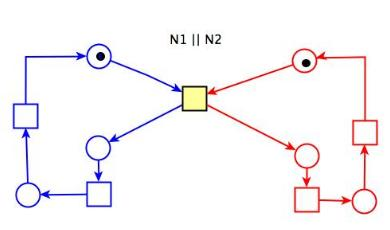
\includegraphics[scale = 0.5]{img/sinc2.jpg} 
  \end{figure}
  La composizione viene indicata con:
  \[N_1||N_2\]
  Lo scatto dell'evento, in maniera sincrona, rende vere le post-condizioni nelle
  due componenti e false le due precondizioni.\\
  Abbiamo appena visto un esempio di \textbf{composizione sincrona}
\end{esempio}
\begin{esempio}
  Supponiamo di avere i modelli di due componenti, $N_1$, che invia in un canale
  un messaggio (per esempio in un buffer), e $N_2$, che riceverà il messaggio
  solo quando esso sarà disponibile:
  \begin{figure}[H]
    \centering
    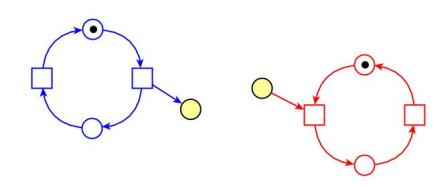
\includegraphics[scale = 0.5]{img/asinc.jpg} 
  \end{figure}
  In questo caso, a differenza dell'esempio precedente, non identifichiamo
  eventi ma condizioni. Identifico quindi il canale (le due condizioni) come uno
  solo, che avrà il pre-evento in una componente e il post-evento nell'altra.\\
  Quindi il pre-evento, nella componente $N_1$, può scattare solo se questa
  nuova condizione condivisa, il canale, è libera, indipendentemente dalla
  componente $N_2$. D'altro canto l'evento in $N_2$ può scattare solo se la
  condizione condivisa è marcata, indipendentemente dallo stato della prima
  componente, liberando il canale di comunicazione.\
  Avvio e ricezione (dopo che il messaggio è stato inviato può essere letto in
  un qualsiasi futuro) non sono sincronizzati e si ha quindi a che fare con
  un esempio di \textbf{composizione asincrona}.\\
  Si avrebbe:
  \begin{figure}[H]
    \centering
    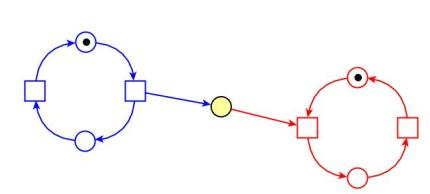
\includegraphics[scale = 0.5]{img/asinc2.jpg} 
  \end{figure}
\end{esempio}
\section{Processi non sequenziali}
 Parliamo ora di sistemi non sequenziali, a ordini parziali (ovvero uno dei tre comportamenti dei sistemi elementari). Difatti Petri voleva \textbf{registrare} il comportamento \textbf{tenendo ben chiare quali fossero le relazioni di dipendenza o indipendenza causale tra gli eventi} (i comportamenti visti fin ora non forniscono tale possibilità). Vediamo un esempio: Petri pensò a un sistema in cui diversi vigili del fuoco, spostandosi avanti nel tempo, che portassero dei secchi per andare a spegnere un fuoco (dato che il sentiero  è
stretto si studia protocollo per cui se hanno il secchio vuoto si muovono a
sinistra fino alla fonte d'acqua e a quel punto ci si sposta a destra). Se due
vigili del fuoco si incontrano lungo la strada si scambiano 
il secchio e invertono la direzione di marcia:
\begin{figure}[H]
  \centering
  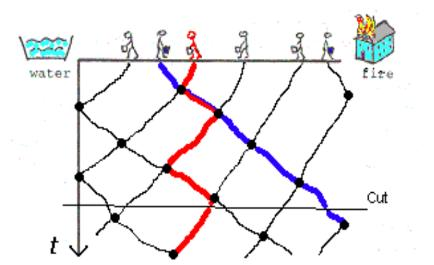
\includegraphics[scale = 0.5]{img/fire.jpg} 
\end{figure}
Un modello classico è quello di far scorrere il tempo come nell'immagine vedendo
gli spostamenti di ogni vigile del fuoco. Nell'immagine si identifica in rosso la storia di
un vigile del fuoco e in blu la storia del secchio pieno.
Ma a Petri non va bene questo modello avendo a che fare col il 
tempo, avendo un modello non discreto.\\
Cerca quindi un modello combinatorio in cui si hanno varie
configurazioni che possono essere osservate (con quindi non necessariamente una
sola scala del tempo).
Si può osservare una configurazione del tipo:
\begin{figure}[H]
  \centering
  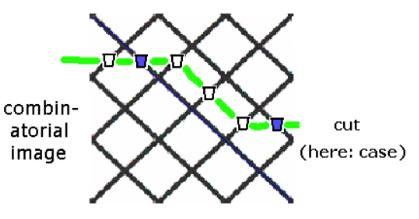
\includegraphics[scale = 0.5]{img/fire2.jpg} 
\end{figure}
con relazioni di dipendenza degli eventi (le righe blu) e situazioni di
indipendenza (la riga verde).
I vigili del fuoco potrebbero essere quindi
modellati da una rete con gli incontri tra vigili del fuoco che diventano
sincronizzazioni. L'evoluzione del sistema può essere registrato salvando
informazioni vere. Nel sistema la prima evento a sinistra è quindi il
prelevamento dell'acqua e l'ultimo a destra il versamento sul fuoco:
\begin{figure}[H]
  \centering
  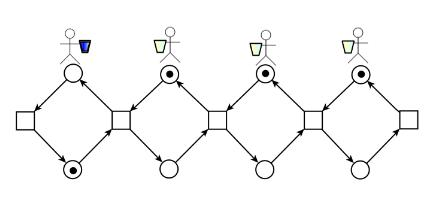
\includegraphics[scale = 0.5]{img/inc.jpg} 
\end{figure}
Gli eventi in mezzo sono i cambiamenti di secchio.\\
L'ordine degli archi segue il secchio, verso sinistra con il secchio vuoto e
verso destra con il secchio pieno. Le condizioni in alto praticamente sono il
secchio vuoto mentre in basso pieno.\\
L'evoluzione del sistema possiamo memorizzarlo tramite condizioni \textbf{vere}. 
\textbf{Possiamo quindi produrre la rete in base alle condizioni che possono scattare}
(in corrispondenza degli elementi della rete),
ottenendo:
\begin{figure}[H]
  \centering
  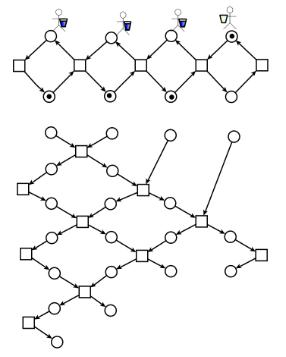
\includegraphics[scale = 0.7]{img/inc2.jpg} 
\end{figure}
Tale modello è infinito.\\
\newpage
Posso modellare i vari percorsi tramite linee colorate (percorso del secchio
pieno in blu, percorso del vigile del fuoco in rosso, secchio vuoto in giallo,
etc$\ldots$) con quelle tratteggiate 
in alto (verde) che rappresentano lo stato iniziale e quelle in basso (viola)
quello finale, dove blocco il sistema
(dopo il quale si ricomincia da capo):
\begin{figure}[H]
  \centering
  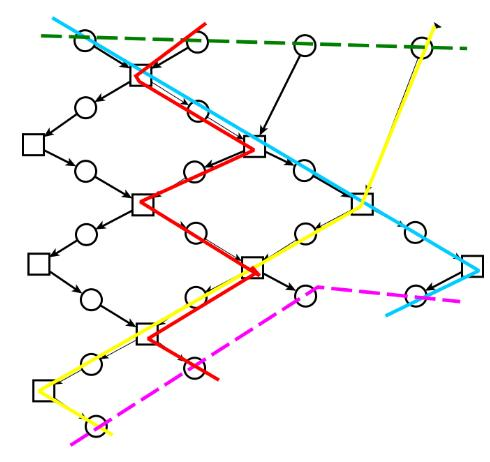
\includegraphics[scale = 0.5]{img/inc3.jpg} 
\end{figure}
Tra le varie linee colorate (non quelle tratteggiate) si hanno relazioni di
dipendenza. \\
\subsection{Reti Causali}
\subsubsection{Introduzione}
Si tratta di particolari reti di petri identificate anche con il nome di \textbf{reti di occorrenze senza conflitti}.
\begin{itemize}
    \item Non ci devono essere cicli
    \item Non ci devono essere conflitti
    \item Preso un qualsiasi evento, il suo passato deve essere finito. L’insieme di elementi che
precedono un evento deve essere finito.
    \item Ad una rete causale è sempre possibile associare un ordine parziale
\end{itemize}
Se $x < y$ possiamo dire che $x$ causa $y$. Grazie a questo possiamo dare la definizione di \textbf{taglio} e \textbf{linea}:
\begin{itemize}
    \item \textbf{TAGLIO}: Data una Rete casuale con un ordinamento parziale, due elementi sono in relazione
\textbf{co} se non è definita una relazione di causalità su di loro (sono causalmente indipendenti). Un
\textbf{co-set} è un insieme di elementi che sono tutti in relazione co. Un taglio non è altro che un co-set massimale.
    \item \textbf{LINEA}: Data una Rete casuale con un ordinamento parziale, due elementi sono in relazione \textbf{li}
se è definito un ordine su di loro, se sono causalmente dipendenti. Un \textbf{li-set} è un insieme di
elementi che sono tutti in relazione li. Una linea non è altro che un li-set massimale.
\end{itemize}
Una rete si dice k-densa se ogni linea ed ogni taglio si intersecano tutti in un punto.
\subsubsection{Definizione}
Definiamo il tutto in modo formale.
\begin{definizione}
  Definiamo:
  \[N=(B, E, F)\]
  come una \textbf{rete causale}, detta anche rete di occorrenze senza conflitti,
  sse:
  \begin{itemize}
    \item $\forall b\in B:|\,^{\bullet}b|\leq 1\land |b^{\bullet}|\leq 1$, ovvero
    non si hanno conflitti, quindi per ogni condizione si ha al più un pre
    evento e un post evento (avendo quindi al più un arco entrante e al più uno
    uscente)
    
    \item $\forall a, y\in B\cup E:(x, y)\in F^+\implies (y, x)\not\in F^+$, ovvero
    non si hanno cicli, quindi presi due elementi collegati da una sequenza di
    archi orientati, avendo un cammino tra i due elementi ($F^+$ è la chiusura
    transitiva della relazione $"F"$) non abbiamo anche un cammino opposto tra i due
    \item $\forall e\in E:\{x\in B\cup E|\, xF^*e\}$ il passato è finito, ovvero si ha un
    numero finito di pre-elementi di un certo elemento
  \end{itemize}
\end{definizione} \vspace{5mm} %5mm vertical space
  Sono quindi reti che registrano un comportamento e quindi non si hanno
  conflitti (che in caso sono sciolti registrando solo quello che è
  effettivamente successo e non quello che potrebbe succedere). Si registra una
  run del sistema. Non si hanno nemmeno cicli perché ogni ripetizione
  dell'evento viene concatenata a quella prima (come detto nell'esempio dopo le
  righe tratteggiate in viola si cominciava da capo).\\
  La rete può essere quindi si infinita ma è composta da un insieme di elementi
  finito che si ripete. In ogni caso il passato di un evento è finito e
  registrato, anche se nel complesso il comportamento è infinito ``in
  avanti''. \\
  Con una rete causale si possono non distinguere più condizioni ed eventi.
\subsubsection{Ordine Parziale delle reti Causali}
Ad una rete causale è possibile associare un ordine parziale:
\[(X,\leq)=(B\cup E, F^*)\]
Dicendo che un elemento ``è minore'' di un altro se esiste un cammino orientato
dall'uno all'altro.
\begin{nota}
$F^*$ non ci farà mai identificare $"x"$ con
$"x"$.
\end{nota}
\begin{esempio}
  Vediamo un esempio di rete causale:
   \begin{figure}[H]
    \centering
    \begin{tikzpicture}[node distance=2cm, bend angle=45, auto]
      \node [place] (p0)  {};
      \node [transitionv] (t1) [right of = p0] {};
      \node [place] (p1) [above right of = t1] {};;
      \node [place] (p2) [below right of = t1] {};
      \node [transitionv] (t2) [right of = p1] {};
      \node [place] (p3) [right of = t2] {}; 
      
      \path[-{Latex[width=2mm]}]
      (p0) edge (t1)
      (t1) edge (p1)
      (t1) edge (p2)
      (p1) edge (t2)
      (t2) edge (p3)
      ;
    \end{tikzpicture}
  \end{figure}
  che quindi avendo un ordine parziale ed essendo causale possiamo scrivere come:
  \begin{figure}[H]
    \centering
    \begin{tikzpicture}[node distance=2cm, bend angle=45, auto]
      \node [place] (p0)  {};
      \node [place] (t1) [right of = p0] {};
      \node [place] (p1) [above right of = t1] {};;
      \node [place] (p2) [below right of = t1, label=below:$"a"$] {};
      \node [place] (t2) [right of = p1, label=above:$"b"$] {};
      \node [place] (p3) [right of = t2] {}; 
      
      \path[-{Latex[width=2mm]}]
      (p0) edge (t1)
      (t1) edge (p1)
      (t1) edge (p2)
      (p1) edge (t2)
      (t2) edge (p3)
      ;
    \end{tikzpicture}
  \end{figure}
  L'ordine \textbf{parziale} si rileva dal fatto che, per esempio, non si ha
  alcuna relazione d'ordine tra $"a"$ e $"b"$.
\end{esempio}
\begin{esempio}
  Vediamo anche due esempi di reti non causali:
  \begin{figure}[H]
    \centering
    \begin{tikzpicture}[node distance=2cm, bend angle=45, auto]
      \node [place] (p0)  {};
      \node [transition] (t1) [right of = p0] {};
      \node [place] (p1) [below of = t1] {};
      \node [transition] (t2) [below of = p1] {};
      \node [place] (p2) [left of = t2] {};
      \node [transition] (t3) [above of = p2] {};
      %\node [place] (p3) [right of = t3] {}; 
      
      \path[-{Latex[width=2mm]}]
      (p0) edge (t1)
      (t1) edge (p1)
      (p1) edge (t2)
      (t2) edge (p2)
      (p2) edge (t3)
      (t3) edge (p0)
      ;
    \end{tikzpicture}
  \end{figure}
  avendo un ciclo.\\
  Oppure:
  \begin{figure}[H]
    \centering
    \begin{tikzpicture}[node distance=2cm, bend angle=45, auto]
      \node [place] (p0)  {};
      \node [transitionv] (t1) [above right of = p0] {};
      \node [transitionv] (t2) [below right of = p0] {};
      \node [place] (p2) [right of = t1] {};
      \node [place] (p3) [right of = t2] {};
      \path[-{Latex[width=2mm]}]
      (p0) edge (t1)
      (p0) edge (t2)
      (t1) edge (p2)
      (t2) edge (p3)
      ;
    \end{tikzpicture}
  \end{figure}
  Avendo un conflitto.
\end{esempio}
\begin{definizione}
  Data una rete causale $N=(B, E, F)$ e dato un ordine parziale $(X, \leq)$ con
  $X=B\cup E$ si ha che si può interpretare la relazione d'ordine come
  indipendenza o dipendenza causale, ovvero presi $x, y\in X$ come elementi che
  occorrono nella storia di $X=B\cup E$ si hanno le seguenti diciture:
  \begin{itemize}
    \item $x \mbox{ \textbf{li} }y$ indica che $x\leq y\lor y\leq x$ e quindi
    corrisponde a \textbf{$"x"$ e $"y"$ sono causalmente dipendenti}. Si ha che
    \textbf{li} può venire letto come \textit{linea} ($"x"$ in linea con $"y"$)
    avendo che uno dei due precede l'altro.  Ovvero si ha una relazione di dipendenza causale tra i due
    \item $x \mbox{ \textbf{co} }y$ indica che $\neg(x< y)\land \neg(y < x)$ e
    quindi corrisponde a \textbf{$"x"$ e $"y"$ sono causalmente indipendenti},
    avendo che i due elementi non si precedono a vicenda, non avendo ordine tra
    loro. Si ha che \textbf{co} sta per \textit{concurrency}
  \end{itemize}
\end{definizione} \vspace{5mm} %5mm vertical space
\begin{esempio}
  Presa la rete causale (già compattata):
  \begin{figure}[H]
    \centering
    \begin{tikzpicture}[node distance=2cm, bend angle=45, auto]
      \node [place] (p0) [label=left:$"a"$] {};
      \node [place] (p1) [above right of = p0, label=above:$"b"$] {};;
      \node [place] (p2) [right of = p0,  label=above:$"c"$] {};
      \node [place] (p3) [right of = p1,  label=right:$"d"$] {}; 
      
      \path[-{Latex[width=2mm]}]
      (p0) edge (p1)
      (p0) edge (p2)
      (p1) edge (p3)
      ;
    \end{tikzpicture}
  \end{figure}
  Si ha che:
  \begin{itemize}
    \item $b \mbox{ \textbf{co} }c$
    \item $c \mbox{ \textbf{co} }d$
    \item $\neg (b \mbox{ \textbf{co} }d)$
    \item $c \mbox{ \textbf{li} }a$
    \item $a \mbox{ \textbf{li} }d$
    \item $\neg (c \mbox{ \textbf{li} }d)$
  \end{itemize}
\end{esempio}
Si ha quindi che \textbf{\textit{li} \textnormal{e} co} sono:
\begin{itemize}
  \item simmetriche
  \item \textbf{non} transitive
  \item riflessive
\end{itemize}
che sono comunque proprietà derivate dalla teoria degli ordini parziali.\\
\subsubsection{Aggiunta della transitività}
Possiamo ora considerare sottoinsiemi dell'ordine parziali in cui la relazione
\textbf{li} e la relazione \textbf{co} sono transitive.
\begin{definizione}[\textbf{Co-Set}]
  Data una rete causale $N=(B, E, F)$ e dato un ordine parziale $(X, \leq)$ con
  $X=B\cup E$ definiamo \textbf{co-set} un sott'insieme di $"X"$:
  \[C\subseteq X\]\mbox{ sse} \[\forall x, y\in C:\, x\mbox{ \textbf{co }}y\]
    Quindi $"C"$ è una clique della relazione \textbf{co}, ovvero tutti gli elementi dell'insieme sono in relazione \textbf{co} tra loro.
\end{definizione} \vspace{5mm} %5mm vertical space
\begin{definizione}[\textbf{Taglio}]
 Data una rete causale $N=(B, E, F)$ e dato un ordine parziale $(X, \leq)$ con
  $X=B\cup E$ definiamo \textbf{taglio} un sott'insieme di $"X"$:
        \[C\subseteq X\]\mbox{ sse }\[C\,\,\,è\,\,\,un\,\,\,co-set\,\,\,massimale.\] Quindi non esiste alcun elemento che, una volta aggiunto, possa andare a creare una relazione \textbf{co} con gli altri elementi precedentemente aggiunti.
        \begin{corollario}
         Si dice \textbf{B-Taglio} un taglio formato interamente da \textbf{condizioni}. Dove ogni elemento è in ha una relazione \textbf{co} con un altro. \textbf{Rappresentano i casi raggiungibili del sistema.}
        \end{corollario}
        \begin{corollario}
         Il taglio ci dice in un certo istante temporale in che stato si trovano tutti i sotto-processi.
        \end{corollario}
 \end{definizione} \vspace{5mm} %5mm vertical space
 \begin{definizione}[\textbf{Li-Set}]
 Data una rete causale $N=(B, E, F)$ e dato un ordine parziale $(X, \leq)$ con
  $X=B\cup E$ definiamo \textbf{li-set} un sott'insieme di $"X"$:
        \[L\subseteq X\]\mbox{ sse }\[ \forall x, y\in L:\, x\mbox{ \textbf{li }}y\]
\end{definizione} \vspace{5mm} %5mm vertical space
 \begin{definizione}[\textbf{Linea}]
 Data una rete causale $N=(B, E, F)$ e dato un ordine parziale $(X, \leq)$ con
  $X=B\cup E$ definiamo \textbf{Linea} un sott'insieme di $"X"$:
        \[L\subseteq X\]\mbox{ sse }\[ L\,\,\,è\,\,\, un\,\,\, li-set\,\,\, massimale\]
        \begin{corollario}
         La linea è la storia di un sotto-processo sequenziale vista come \textit{"parto da un certo stato che è la configurazione di condizioni vere iniziale e vedo cosa succede a partire da qui durante la run (quindi non vedo l'esecuzione concorrente ma solo quella di un sotto-processo)"}
        \end{corollario}
\end{definizione} \vspace{5mm} %5mm vertical space
\begin{nota}
In un \textbf{co-set} la relazione \textbf{co} è \textbf{transitiva}
\end{nota}

\begin{nota}
In un \textbf{li-set} la relazione \textbf{li} è \textbf{transitiva}
\end{nota}
\begin{nota}
Linee e tagli possono essere sia eventi che condizioni.
\end{nota}
\begin{esempio}
  Tornando all'esempio del secchio:
  \begin{figure}[H]
    \centering
    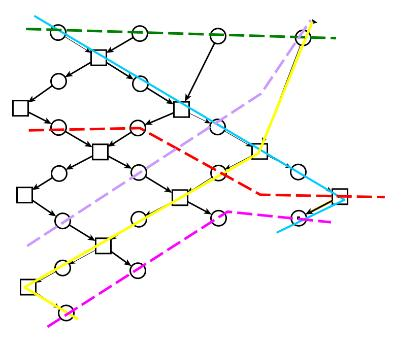
\includegraphics[scale = 0.5]{img/ta.jpg} 
  \end{figure}
  si ha che:
  \begin{itemize}
    \item la storia del secchio è un insieme di elementi in relazione
    \textbf{li} e, nello specifico, ad esempio la parte azzurra o quella gialla,
    è una \textit{linea} che descrive un sotto-processo
    \item le parti tratteggiate, sono invece
    un co-set e, nel dettaglio, sono un 
    taglio (infatti se cerco di aggiungere un qualsiasi altro elemento otterrei
    una relazione di dipendenza con uno degli elementi già presenti)
  \end{itemize}
\end{esempio}
\begin{nota}
I tagli fatti di sole condizioni rappresentano casi raggiungibili
  (nell'immagine quello verde che quello viola che quello viola-chiaro)
\end{nota}
Una rete causale quindi registra il comportamento di un sistema elementare.\\
Si hanno quindi, con i tagli, possibili osservazioni di configurazioni possibili
nella storia del sistema. In particolare, una rete causale, non registra cosa succede al variare del tempo ma registra le varie dipendenze e indipendenze causali tra le condizioni e gli eventi che occorrono.
\begin{definizione}
  Grazie alle reti causali, preso un elemento $x\in X$, possiamo definire:
  \begin{itemize}
    \item $past(x)$, ovvero il passato dell'elemento, tutti gli elementi in
    relazione $\leq$ di $"x"$
    \item $future(x)$, ovvero il futuro dell'elemento, tutti gli elementi in
    relazione $\geq$ di $"x"$
  \end{itemize}
  Visualizzabili, per esempio, nell'immagine, rispettivamente in rosso e blu:
  \begin{figure}[H]
    \centering
    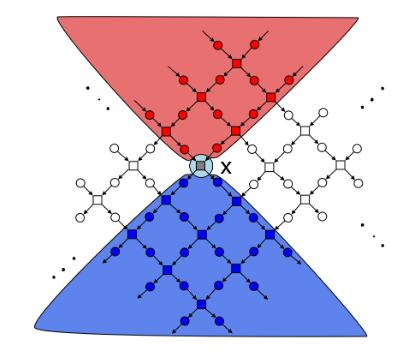
\includegraphics[scale = 0.5]{img/pf.jpg} 
  \end{figure}
  Gli elementi nell'anti-cono (la parte bianca) sono in relazione \textbf{co}
  con $"x"$ e quindi possono essere concorrenti.
\end{definizione} \vspace{5mm} %5mm vertical space
\subsubsection{K-Densità}
\begin{definizione}
  Data una rete causale $N=(B, E, F)$ e dato un ordine parziale $(X, \leq)$ con
  $X=B\cup E$ definiamo che la rete è \textbf{K-densa} se ogni linea e ogni
  taglio si intersecano tutti in un punto, ovvero: tutti hanno un punto comune. Formalmente:
  \[\forall\, h\in Linee(N),\forall\, c\in Tagli(N):|h\cap c|=1\]
  Con $Linee(N)$ e $Tagli(N)$ che sono rispettivamente gli insiemi di tutte le
  linee e dei tagli.\\
  \end{definizione} \vspace{5mm} %5mm vertical space
  Quindi per ogni coppia Taglio-Linea, se la linea rappresenta un sotto-processo e il taglio rappresenta una \textit{"fotografia"} di quello che sta succedendo, allora ogni sotto-processo deve incrociarci con quello che viene fotografato.
  \begin{nota}
  Immaginiamo una linea come la "storia" di un sotto-processo. Quindi viene interpretata come un sotto-processo sequenziale. Mentre una fotografia su una linea indica che un sotto-processo si deve trovare in un qualche stato.
  \end{nota}
\begin{nota}
Ogni rete che modella il comportamento di un sistema deve essere k-densa.
\end{nota}
  \begin{nota}
  Se $"N"$ è finita è anche \textbf{K-densa}, se sono infinite non è detto.
\end{nota}
  \begin{esempio}
  Una rete non K-densa potrebbe essere (in rosso una linea e in blu un taglio):
  \begin{figure}[H]
    \centering
    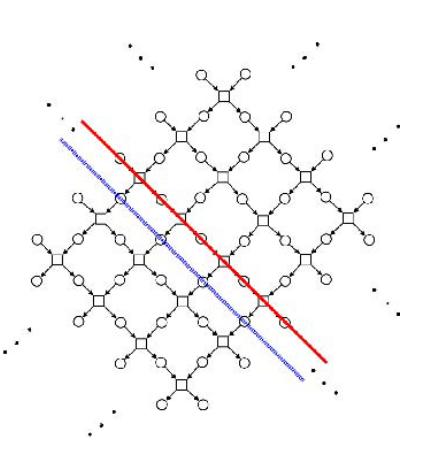
\includegraphics[scale = 0.36]{img/de1.jpg} 
  \end{figure}
  (si nota che è una rete infinita).\\
  e una K-densa:
  \begin{figure}[H]
    \centering
    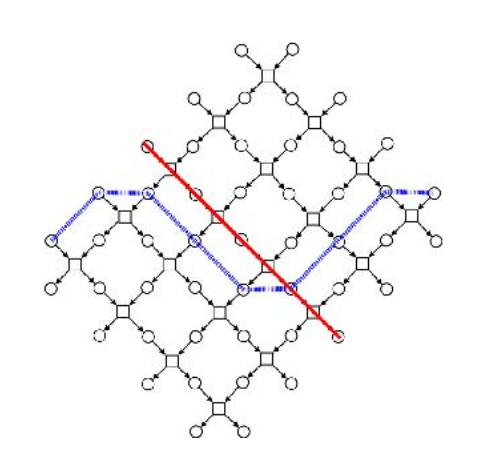
\includegraphics[scale = 0.36]{img/de2.jpg} 
  \end{figure}
  (si nota che è una rete finita).\\
  ($"K"$ significa combinatoria).
\end{esempio}
\begin{esempio}
  Vediamo anche il solito esempio della mutua esclusione:
  \begin{figure}[H]
    \centering
    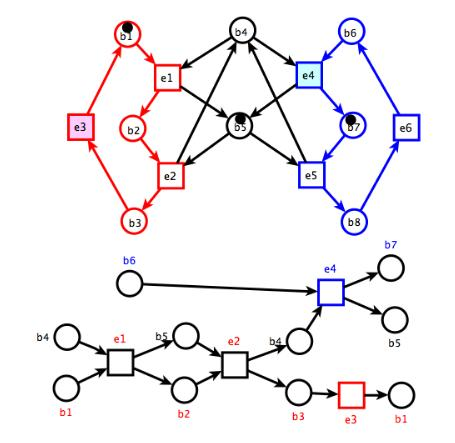
\includegraphics[scale = 0.5]{img/de3.jpg} 
  \end{figure}
  Consideriamo sia il sistema elementare che la rete causale associata (dove si vede ad
  esempio che $e_4$ ed $e_3$ sono in relazione \textbf{co}, le prime tre
  condizioni a sinistra ($b_1, b_4, b_6$) sono un taglio anche le
  ultime a destra ($b_1, b_5, b_7$)). 
\end{esempio}
\subsection{Processi non sequenziali - Definizione}
Dato un sistema elementare senza conflitti e finito, possiamo dire che P è un processo di questa rete
se la rete del processo è una rete causale e ci fa corrispondere eventi/condizioni del sistema in
eventi/condizioni della rete. Se registriamo un evento devo essere sicuro di registrare tutte le sue pre
e le sue post. Tramite questa procedura ci assicuriamo di registrare un'esecuzione del sistema (ma non tutte), ovvero solo le dipendenze e indipendenze causali.
\begin{definizione}
  Sia $\Sigma=(S, T, F, c_{in})$ un sistema elementare senza contatti e finito,
  tale che $S\cup T$ sia finito. Si ha che, con $\phi$ che mappa dalla rete
  causale al sistema elementare: 
  \[\langle N=(B, E, F), \phi\rangle\]
  è un processo non sequenziale di $\Sigma$ sse:
  \begin{itemize}
    \item $(B, E, F)$ è una rete causale (si ammettono condizioni isolate)
    \item $\phi:B\cup E\to S\cup T$ è una mappa tale che:
    \begin{itemize}
      \item $\phi(B)\subseteq S, \phi(E)\subseteq T$
      \item $\forall x, y\in B\cup E:\phi(x)=\phi(y)\implies (x\leq y)\lor (y\leq
      x)$ Due elementi mappati sullo stesso elemento del sistema, allora saranno registrazioni dello stessa condizione/evento in successione per due volte. Allora sicuramente una delle due condizioni deve essere minore dell'altra perchè viene registrata prima. Non avendo quindi concorrenza. In particolare i due $x,y$ saranno in relazione \textbf{li}.
      \item $\forall e\in E:\phi(\,^\bullet e)=\,^\bullet
      \phi(e)\land\phi(e^\bullet)=\phi(e)^\bullet$ quindi le precondizioni di un
      evento nella rete causale devono corrispondere alle pre dell'evento nel
      sistema elementare (e così anche per le post). Ovvero si devono registrare tutte le "pre" e tutte le "post" del sistema.
      \item $\phi(Min(N))=c_{in}$,\\ con $Min(N)=\{x\in B|\nexists
      y: (y, x)\in F\}$ 
      Le condizioni iniziali (minimali rispetto alla relazione d'ordine), corrispondano al caso iniziale del sistema. Si prendono gli elementi che non hanno archi entranti nella rete, (che saranno condizioni poiché è un sistema senza contatti) queste condizioni verranno mappate nel caso iniziale. Dobbiamo avere la registrazione del caso iniziale. Ovvero: l'immagine delle condizioni deve essere il caso iniziale.
      \begin{nota}
      Non possiamo avere $x\in E$ poiché gli eventi senza archi entranti sono eventi senza pre-condizioni. Allora sicuramente avremo le pre-condizioni vere (poiché vuote) ma le post non tutte false. Quindi si avrebbero dei contatti.
      \end{nota}
    \end{itemize}
  \end{itemize}
  \begin{figure}[H]
          \centering
          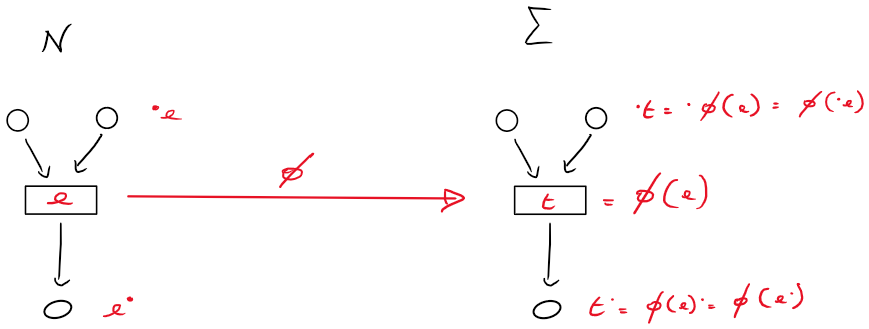
\includegraphics[width=0.7\textwidth]{img/procnonseq.png}      
          \end{figure}
  Se abbiamo queste proprietà la rete causale è una registrazione del sistema
  elementare.\\
  In tal caso si ha che $N=(B, E, F)$ è K-densa (sia che sia finita che infinita),
  avendo il sistema di partenza finito. Le linee sono quindi sotto-processi
  sequenziali e i tagli possibili configurazioni sempre raggiungibili.\\
  Inoltre si ha che:
  \[\forall K\in B\mbox{ K è B-taglio di } N \mbox{ t.c. } K \mbox{ è finito}
    \land \exists c\in C_\Sigma:\phi(K)=c\]
\end{definizione} \vspace{5mm} %5mm vertical space


\subsection{Registrazione di più run del sistema}
Dato un sistema abbiamo tanti processi non sequenziali che rappresentano esecuzioni
del sistema. In particolare:
\begin{definizione}
  Se un sistema presenta dei conflitti, possiamo avere diversi modi per risolverli. Ogni modo differente presenta una differente run del sistema.
\end{definizione}
Ci si chiede quindi se abbiamo un unico oggetto che rappresenta tutti i
possibili run del sistema. Questo oggetto esiste e sono i \textbf{processi ramificati}, ma per introdurli dobbiamo prima parlare di \textbf{reti di occorrenze}.
\begin{figure}[H]
  \centering
  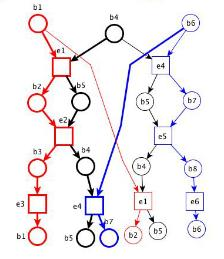
\includegraphics[scale = 0.6]{img/be4.jpg}
  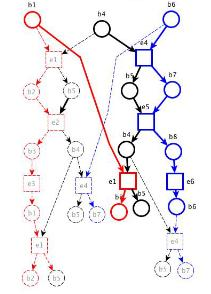
\includegraphics[scale = 0.6]{img/be5.jpg} 
  \caption{Esempio con più processi del modello della mutua esclusione
    modellati da un’unica rete con conflitti in avanti.}
\end{figure}
\subsubsection{Reti di Occorrenze}
Una rete di occorrenze è una particolare rete, utilizzata \textbf{al posto delle reti causali}, tale che:
\begin{itemize}
    \item Ha conflitti solo in avanti.
    \item Non ci sono cicli.
    \item Il passato di un
evento è finito.
    \item La relazione di conflitto non è riflessiva.
\end{itemize}
\begin{definizione}
  Data una rete causale $N=(B, E, F)$, con $X=B\cup E$, diciamo che è una
  \textbf{rete di occorrenze} sse:
  \begin{itemize}
    \item $\forall\, b\in B:|\,^\bullet b|=1$, I pre eventi di ogni condizione sono al più uno.Ovvero abbiamo conflitti solo in
    avanti
    \item $\forall\, x, y\in B\cup E:(x, y)\in F^+\implies (y, x)\not\in F^+$,
    ovvero non abbiamo cicli, in quanto le ripetizioni sono già registrate
    \item $\forall\, e\in E:\{x\in B\cup E|xF^*e\}$, ovvero il passato di un
    evento, è finito 
    \item la \textbf{relazione di conflitto} $\#$ \textbf{non è riflessiva}, avendo:
    \[\#\subset X\times X\]
    definita come:
    \[x\# y\iff \exists e_1, e_2\in E:\,^\bullet e_1\cap \,^\bullet e_2\neq
      \emptyset \land e_1\leq x\land e_2\leq y\]
    ovvero due elementi sono in conflitto sse sono in ``alternativa'' ovvero se
    si hanno due eventi che condividono precondizioni (sicuramente non le post
    non avendo conflitti in avanti) con i due eventi che causano i due elementi
    $"x"$ e $"y"$, allora anche questi due sono in conflitto. Vediamo degli esempi:
    \begin{figure}[H]
      \centering
      \begin{tikzpicture}[node distance=1.7cm, bend angle=45, auto]
        \node [place] (p0)  {};
        \node [transitionv] (t1) [above right of = p0] {};
        \node [transitionv] (t2) [below right of = p0] {};
        \node [place] (p2) [right of = t1] {};
        \node [place] (p3) [above right of = t2] {};
        \node [place] (p4) [right of = t2, label=below:$"x"$] {};
        \node [transitionv] (t3) [right of = p2, label=above:$"y"$] {};
        \node [place] (p5) [right of = t3] {};
        % \node [place] (p3) [right of = t3] {}; 
        
        \path[-{Latex[width=2mm]}]
        (p0) edge (t1)
        (p0) edge (t2)
        (t1) edge (p2)
        (p2) edge (t3)
        (t3) edge (p5)
        (t2) edge (p3)
        (t2) edge (p4)
        ;
      \end{tikzpicture}
      \caption{Esempio con $"x"$ e $"y"$ non in conflitto. Nel dettaglio questa è
        una rete di occorrenze}
      \label{fig:esemp}
    \end{figure}
    \begin{figure}[H]
      \centering
      \begin{tikzpicture}[node distance=1.7cm, bend angle=45, auto]
        \node [place] (p0) [label=left:$"p"$] {};
        \node [transitionv] (t1) [above right of = p0, label=above:$e_1$] {};
        \node [transitionv] (t2) [below right of = p0, label=below:$e_2$] {};
        \node [place] (p2) [right of = t1] {};
        \node [place] (p3) [above right of = t2] {};
        \node [place] (p4) [right of = t2] {};
        \node [transitionv] (t3) [right of = p2, label=above:$"z"$] {};
        \node [place] (p5) [right of = t3] {};
        % \node [place] (p3) [right of = t3] {}; 
        
        \path[-{Latex[width=2mm]}]
        (p0) edge (t1)
        (p0) edge (t2)
        (t1) edge (p2)
        (p2) edge (t3)
        (t3) edge (p5)
        (p3) edge (t3)
        (t2) edge (p3)
        (t2) edge (p4)
        ;
      \end{tikzpicture}
      \caption{Esempio con $"z"$ che è in conflitto con se stessa (avendo $e_1<z$
        e $e_2<z$, con i due eventi che condividono $"p"$) e quindi non può
        essere una rete di occorrenze}
    \end{figure}
  \end{itemize}
  È comunque possibile associare a una rete di occorrenze $"N"$ un ordine
  parziale.
  \begin{definizione}
    La relazione di conflitto non può avvenire se esistono relazioni \textbf{li} o \textbf{co} tra gli elementi corrispondenti.
  \end{definizione}
\end{definizione} \vspace{5mm} %5mm vertical space
\subsubsection{Processi Ramificati}
Un processo si dice ramificato quando si sono registrati piu comportamenti in una rete, la rete che
mi registra tutti i comportamenti si chiama \textbf{unfolding} (piu precisamente possiamo dire che l’unfolding
rappresenta il processo ramificato che contiene tutti i comportamenti del sistema). Un processo
ramificato è definito con una rete di occorrenze.
Prendiamo in considerazione tutti i possibili comportamenti di un sistema. Per far ciò sfruttiamo un \textbf{Processi Ramificato}, ovvero un'\textbf{alternativa} alle reti causali. Per cui un processo deve descrivere fino a un certo punto cosa è successo, ma descriviamo tutti i possibili futuri. Quindi parliamo della registrazione dei possibili futuri di un processo, dove vi sono solo conflitti in avanti. Molto utili in questo ambito sono le \textbf{reti di occorrenza}, che hanno il compito di registrare tutti i possibili processi \textbf{non} sequenziali dove i conflitti sono \textbf{solo} in avanti.
\begin{definizione}
  Sia $\Sigma=(S, T, F, c_{in})$ un sistema elementare senza contatti e
  finito. Si ha che:
  \[\langle N=(B, E, F), \phi\rangle\]
  è un \textbf{processo ramificato} di $\Sigma$ sse:
  \begin{itemize}
    \item $(B, E, F)$ è una rete di occorrenze (si ammettono condizioni isolate,
    volendo poter registrare il caso iniziale come un insieme di condizioni che
    magari non vengono modificate)
    \item $\phi:B\cup E\to S\cup T$ è una mappa tale che:
    \begin{itemize}
      \item $\phi(B)\subseteq S, \phi(E)\subseteq T$
      \item $\forall e_1, e_2\in E:(\,^\bullet e_1=\,^\bullet e_2\land
      \phi(e_1)=\phi(e_2))\implies e_1=e_2$, ovvero se due eventi condividono le
      precondizioni e corrispondono allo stesso evento del sistema (secondo la
      mappa) allora necessariamente sono lo stesso evento. Quindi non necessariamente possiamo registrare due eventi perchè sono in linea, come nelle reti causali, ma perchè possono essere anche in conflitto. Questo può avvenire perchè siamo in un processo ramificato.
      \item $\forall e\in E:\phi(\,^\bullet e)=\,^\bullet
      \phi(e)\land\phi(e^\bullet)=\phi(e)^\bullet$ quindi le precondizioni di un
      evento nella rete di occorrenze devono corrispondere alle pre dell'evento nel
      sistema elementare (e così anche per le post). Ovvero dobbiamo registrare tutte le "pre" e tutte le "post". 
      \begin{nota}
        In realtà deve esserci una corrispondenza biunivoca tra le precondizioni della rete e quelle del sistema. Quindi \textbf{non} possiamo mappare più precondizioni della rete in \textbf{una sola } precondizione del sistema e viceversa.
      \end{nota}
      \item $\phi(Min(N))=c_{in}$, quindi il taglio iniziale deve essere il caso
      iniziale del sistema. In particolare ci vuole una relazione biunivoca tra $(Min(N))$ e $c_{in}$.
    \end{itemize}
  \end{itemize}
\end{definizione} \vspace{5mm} %5mm vertical space
\begin{esempio}
  Riprendendo il solito esempio di mutua esclusione:
  \begin{figure}[H]
    \centering
    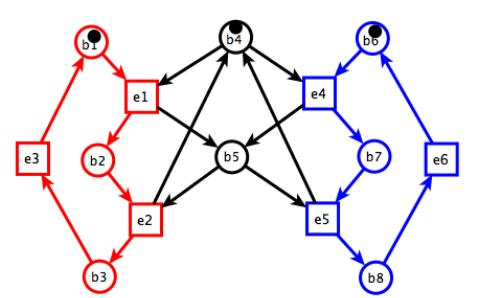
\includegraphics[scale = 0.45]{img/ram0.jpg} 
  \end{figure}
  \newpage
  si ha il seguente processo ramificato:
  \begin{figure}[H]
    \centering
    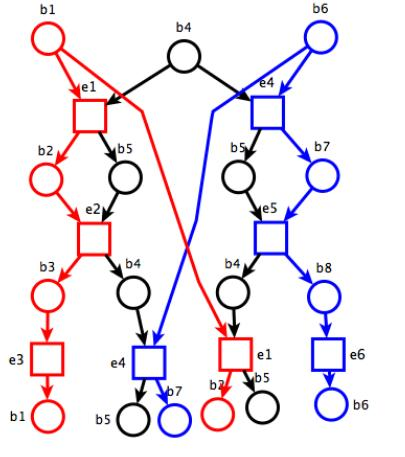
\includegraphics[scale = 0.45]{img/ram.jpg} 
  \end{figure}
  
\end{esempio}
\noindent
Cerchiamo ora di definire meglio l'unfolding, quell'oggetto che rappresenta
tutti i possibili sotto-processi non sequenziali del sistema, ovvero tutti i
possibili comportamenti del sistema.\\
Definiamo prima dei ``prerequisiti''.
\begin{definizione}[Prefisso]
  Sia $\Sigma=(S, T, F, c_{in})$ un sistema elementare senza contatti e finito, e
  siano:
  \[\Pi_1=\langle N_1;\phi_1\rangle\]
  \[\Pi_2=\langle N_2;\phi_2\rangle\]
  due processi ramificati di $\Sigma$.\\
  Si ha che $\Pi_1$ è un \textbf{prefisso} di $\Pi_2$ (e quindi $\Pi_1$ è un
  sotto-processo di $\Pi_2$) sse:
  \begin{itemize}
    \item $N_1$ è una sottorete di $N_2$
    \item $\phi_{2|N_1}=\phi_1$ ovvero $\phi_2$ ristretto a $N_1$  è uguale a
    $\phi_1$ 
  \end{itemize}
  Questo vuol dire che $N_2$ registra tutto quello che registra $N_1$ e anche qualcos'altro.
  \end{definizione}
  \begin{figure}[H]
    \centering
    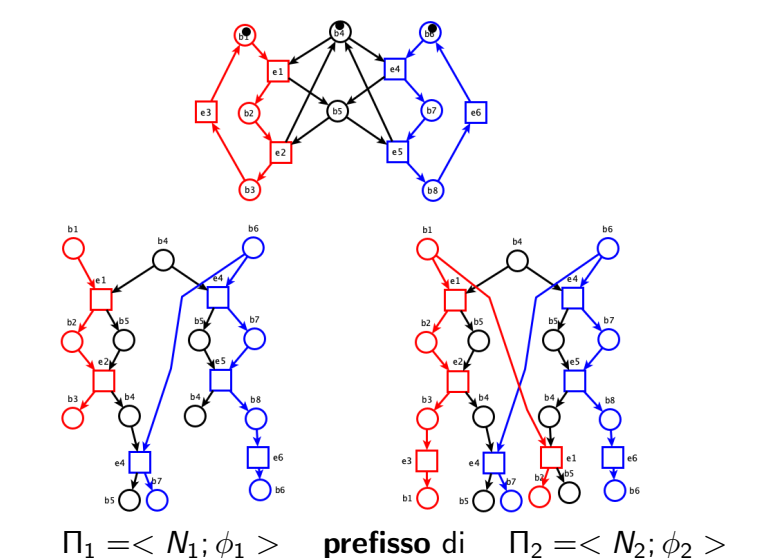
\includegraphics[width=1\textwidth]{img/prefisso.png}
\end{figure}
  \begin{definizione}[Unfolding]
  Si ha che $\Sigma$ ammette un unico processo ramificato che è massimale
  rispetto alla relazione di prefisso tra processi e tale processo è detto
  \textbf{unfolding} di $\Sigma$:
  \[Unf(\Sigma)\]
  \begin{corollario}
   Un processo ramificato è un prefisso dell'unfolding.
  \end{corollario}
  \begin{nota}
    Quindi è il processo ramificato più grande tale per cui tutti gli altri saranno \textbf{prefissi} di questo.
  Esso può essere infinito se il sistema ha comportamento ciclico.
  \end{nota}
  \begin{nota}
  Ha senso studiare un prefisso finito dell'unfolding che permette di
  determinare tutto l'unfolding.
  \end{nota}
  \begin{nota}
    L'unfolding tiene traccia di tutti i processi sequenziali di un sistema
  elementare. 
  \end{nota}
\end{definizione} \vspace{5mm} %5mmvertical space
\begin{definizione}
  Un \textbf{processo non sequenziale} è un processo ramificato
  $\Pi=\langle N;\phi\rangle$
  tale che $"N"$ è una rete causale (senza conflitti). Il processo $\Pi$ è anche
  detto \textbf{run}/\textbf{corsa} di $"N"$.
  \begin{corollario}
   Ogni processo non sequenziale di $\Sigma$ è un prefisso dell'unfolding $Unf(\Sigma)$
  \end{corollario}
\end{definizione}

\begin{esempio}
  Riprendendo il solito esempio di mutua esclusione si ha il seguente unfolding
  infinito:
  \begin{figure}[H]
    \centering
    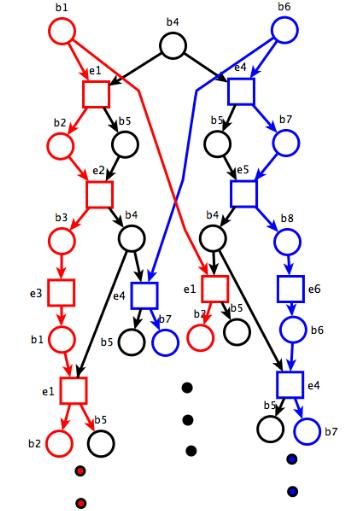
\includegraphics[scale = 0.45]{img/unf.jpg} 
  \end{figure}
\end{esempio}
Si è cercato di capire se un prefisso dell'unfolding basti a studiare l'intero
sistema. Tale problema lo si risolve mediante i prefissi completi.
\begin{definizione}
  Definiamo \textbf{prefisso completo} un prefisso che include tutti i casi (o finito)
  raggiungibili.
\end{definizione} \vspace{5mm} %5mm vertical space
% \subsection{Reti posti e transizioni}
% Vediamo ora una nuova classe delle \textit{reti di Petri}, detta \textbf{reti
% Posti e Transizioni}, permette di rappresentare un sistema in modo più
% compatto, sono una sorta di \textit{ripiegamento} dei sistemi
% elementari. Partiamo quindi da un esempio:
% \begin{esempio}
%   prendiamo in studio sempre il sistema produttore-consumatore:
%   Sia nella versione con contatto:
%   \begin{figure}[H]
%     \centering
%     \begin{tikzpicture}[node distance=2cm, bend angle=45, auto]
%       \node [place, tokens=1] (p0) [label=above:\small{P2}] {};
%       \node [transition] (t1) [below right of = p0, label=left:\small{d}] {};
%       \node [transition] (t2) [below left of = p0, label=left:\small{p}] {};
%       \node [place] (p1) [below right of = t2, label=below:\small{P1}] {}; 
%       \node [place, tokens=1] (p3) [right of = t1, label=above:\small{B}] {};
%       \node [transition] (t4) [right of = p3, label=right:\small{e}] {};

%       \node [place, tokens=1] (p2) [above right of = t4, label=above:\small{C1}] {}; 
%       \node [transition] (t3) [below right of = p2, label=right:\small{c}] {};
%       \node [place] (p4) [below right of = t4, label=below:\small{C2}]
%       {}; 

%       \path[-{Latex[width=2mm]}]
%       (p0) edge (t1)
%       (t1) edge (p1)
%       (p1) edge (t2)
%       (t2) edge (p0)
%       (t1) edge (p3)
%       (p3) edge (t4)
%       (t4) edge (p4)
%       (p4) edge (t3)
%       (t3) edge (p2)
%       (p2) edge (t4)
%       ;
%     \end{tikzpicture}
%   \end{figure}
%   che senza:
%   \begin{figure}[H]
%     \centering
%     \begin{tikzpicture}[node distance=2cm, bend angle=45, auto]
%       \node [place, tokens=1] (p0) [label=above:\small{P2}] {};
%       \node [transition] (t1) [below right of = p0, label=left:\small{d}] {};
%       \node [transition] (t2) [below left of = p0, label=left:\small{p}] {};
%       \node [place] (p1) [below right of = t2, label=below:\small{P1}] {}; 
%       \node [place, tokens=1] (p31) [above right  of = t1, label=above:\small{B1}] {};
%       \node [place] (p32) [ below right of = t1, label=below:\small{B2}] {};
%       \node [transition] (t4) [below right of = p31, label=right:\small{e}] {};

%       \node [place, tokens=1] (p2) [above right of = t4, label=above:\small{C1}] {}; 
%       \node [transition] (t3) [below right of = p2, label=right:\small{c}] {};
%       \node [place] (p4) [below right of = t4, label=below:\small{C2}]
%       {}; 

%       \path[-{Latex[width=2mm]}]
%       (p0) edge (t1)
%       (t1) edge (p1)
%       (p1) edge (t2)
%       (t2) edge (p0)
%       (t1) edge (p32)
%       (p32) edge (t4)
%       (t4) edge (p31)
%       (p31) edge (t1)

%       (t4) edge (p4)
%       (p4) edge (t3)
%       (t3) edge (p2)
%       (p2) edge (t4)
%       ;
%     \end{tikzpicture}
%   \end{figure}
%   Suppongo di voler modellare il sistema in modo che il buffer possa avere un
%   numero determinato di posizioni, per esempio 2 (il buffer può quindi
%   depositare fino a due elementi). Si ottiene quindi:
%   \begin{figure}[H]
%     \centering
%     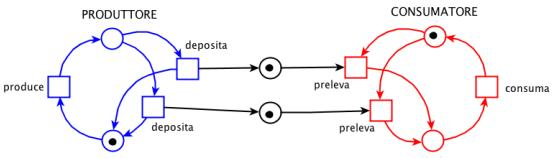
\includegraphics[scale = 0.6]{img/pt3.jpg} 
%   \end{figure}
%   Dove si hanno due posizioni del buffer (e quindi basta che una sia vuota per
%   permettere al produttore di depositare) a disposizione del sistema. Si nota
%   come l'aumento dei buffer complica drasticamente la modellazione del sistema.
%   Si cerca quindi una soluzione più compatta, compattando gli eventi
%   \textit{deposita} e \textit{preleva} e dando nuova notazione al buffer. Si
%   ottiene:
%   \begin{figure}[H]
%     \centering
%     \begin{tikzpicture}[node distance=2cm, bend angle=45, auto]
%       \node [place] (p0) [label=above:\small{P2}] {};
%       \node [transition] (t1) [below right of = p0, label=left:\small{d}] {};
%       \node [transition] (t2) [below left of = p0, label=left:\small{p}] {};
%       \node [place, tokens = 1] (p1) [below right of = t2, label=below:\small{P1}] {}; 
%       \node [place, tokens=2] (p3) [right of = t1, label=above:$\mbox{B,
%         capacità=2}$] {}; 
%       \node [transition] (t4) [right of = p3, label=right:\small{e}] {};

%       \node [place, tokens=1] (p2) [above right of = t4, label=above:\small{C1}] {}; 
%       \node [transition] (t3) [below right of = p2, label=right:\small{c}] {};
%       \node [place] (p4) [below right of = t4, label=below:\small{C2}]
%       {}; 
      
%       \path[-{Latex[width=2mm]}]
%       (p0) edge (t1)
%       (t1) edge (p1)
%       (p1) edge (t2)
%       (t2) edge (p0)
%       (t1) edge (p3)
%       (p3) edge (t4)
%       (t4) edge (p4)
%       (p4) edge (t3)
%       (t3) edge (p2)
%       (p2) edge (t4)
%       ;
%     \end{tikzpicture}
%   \end{figure}
%   con il buffer che diventa anche un \textbf{contatore} del numero di elementi
%   presenti al suo interno. Un buffer a due posizioni diventa quindi una
%   condizione non più booleana, detta \textbf{Posto}, con una \textbf{capacità}
%   pari a 2. Il produttore non può produrre oltre la capacità.\\
%   Con questa rappresentazione non abbiamo più alcuna difficoltà nel rappresentare più
%   posizioni del buffer in quanto basta aumentare la capacità. abbiamo però perso
%   delle informazioni infatti non abbiamo più una relazione di dipendenza tra dove si
%   deposita (se nella prima posizione o nella seconda) e dove si preleva.\\
%   Aggiungiamo un'altra complicanza: aggiungiamo un secondo consumatore:
%   \begin{figure}[H]
%     \centering
%     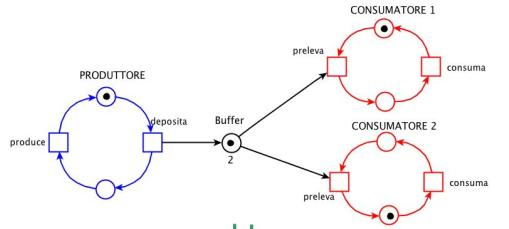
\includegraphics[scale = 0.6]{img/pt5.jpg} 
%   \end{figure}
%   Possiamo \textit{comprimere} nella stessa maniera, ottenendo, in quanto i due
%   consumatori hanno lo stesso modello di comportamento:
%   \begin{figure}[H]
%     \centering
%     \begin{tikzpicture}[node distance=2cm, bend angle=45, auto]
%       \node [place] (p0) [label=above:\small{P2}] {};
%       \node [transition] (t1) [below right of = p0, label=left:\small{d}] {};
%       \node [transition] (t2) [below left of = p0, label=left:\small{p}] {};
%       \node [place, tokens = 1] (p1) [below right of = t2, label=below:\small{P1}] {}; 
%       \node [place, tokens=1] (p3) [right of = t1, label=above:\small{B}] {};
%       \node [transition] (t4) [right of = p3, label=right:\small{e}] {};

%       \node [place, tokens=1] (p2) [above right of = t4, label=above:\small{C1}] {}; 
%       \node [transition] (t3) [below right of = p2, label=right:\small{c}] {};
%       \node [place, tokens =1] (p4) [below right of = t4, label=below:\small{C2}]
%       {}; 
      
%       \path[-{Latex[width=2mm]}]
%       (p0) edge (t1)
%       (t1) edge (p1)
%       (p1) edge (t2)
%       (t2) edge (p0)
%       (t1) edge (p3)
%       (p3) edge (t4)
%       (t4) edge (p4)
%       (p4) edge (t3)
%       (t3) edge (p2)
%       (p2) edge (t4)
%       ;
%     \end{tikzpicture}
%   \end{figure}
%   Anche qui perdo l'informazione riguardo quale dei due consumatori ha
%   effettivamente prelevato, riguardo quale dei due è pronto a \textit{prelevare}
%   e quale a \textit{consumare}, continuando ad ignorare anche la posizione
%   del buffer nei confronti della quale stanno agendo.\\
%   Si può arrivare ad avere due componenti identiche che sono concorrenti tra
%   loro. 
% \end{esempio}
% Le condizioni non sono più, in generale, booleane ma sono \textbf{posti}
% dotati di \textbf{contatori}, gli elementi all'interno sono detti
% \textbf{marche}. Ai posti si assegna anche una \textbf{capacità}. 
% \\
% Si ha inoltre che lo scatto di una evento dipende dalla disponibilità
% delle risorse, per esempio un produttore può produrre $"n"$ elementi alla volta
% e il consumatore consumarne $"m"$. Si usano quindi archi pesati (se non indicato
% ovviamente ha peso 1, quello del normale check booleano di condizione attiva)
% tali che una evento possa scattare sse i pesi vengono rispettati:
% \begin{figure}[H]
%   \centering
%   \begin{tikzpicture}[node distance=2cm, bend angle=45, auto]
%     \node [transition] (t0) [label=left:$t_1$] {};
%     \node [place] (p0) [above left of = t0, label=above:\small{P0}] {};       
%     \node [place, tokens = 6, minimum size = 0.9cm] (p1) [above right of = t0, label=above:\small{P1}] {}; 
%     \node [place] (p2) [below left of = t0, label=below:\small{P2}] {}; 
%     \node [place] (p3) [below of = t0, label=below:\small{P3}] {}; 
%     \node [place] (p4) [below right of = t0, label=below:\small{P4}] {}; 

%     {}; 
    
%     \path[-{Latex[width=2mm]}]
%     (p0) edge (t0)
%     (p1) edge node {5} (t0)
%     (t0) edge (p2)
%     (t0) edge node {2}(p3)
%     (t0) edge (p4)
%     ;
%   \end{tikzpicture}
%   \qquad\qquad\qquad
%   \begin{tikzpicture}[node distance=2cm, bend angle=45, auto]
%     \node [transition] (t0) [label=left:$t_1$] {};
%     \node [place, tokens = 2] (p0) [above left of = t0, label=above:\small{P0}] {};       
%     \node [place, tokens = 4, minimum size = 0.7cm] (p1) [above right of = t0, label=above:\small{P1}] {}; 
%     \node [place] (p2) [below left of = t0, label=below:\small{P2}] {}; 
%     \node [place] (p3) [below of = t0, label=below:\small{P3}] {}; 
%     \node [place] (p4) [below right of = t0, label=below:\small{P4}] {}; 

%     {}; 
    
%     \path[-{Latex[width=2mm]}]
%     (p0) edge (t0)
%     (p1) edge node {5} (t0)
%     (t0) edge (p2)
%     (t0) edge node {2}(p3)
%     (t0) edge (p4)
%     ;
%   \end{tikzpicture}
%   \caption{Esempi con la evento $t_i$ non abilitata}
% \end{figure}
% \begin{figure}[H]
%   \centering
%   \begin{tikzpicture}[node distance=2cm, bend angle=45, auto]
%     \node [transition] (t0) [label=left:$t_1$] {};
%     \node [place, tokens = 2] (p0) [above left of = t0, label=above:\small{P0}] {};       
%     \node [place, tokens = 5, minimum size = 0.7cm] (p1) [above right of = t0, label=above:\small{P1}] {}; 
%     \node [place] (p2) [below left of = t0, label=below:\small{P2}] {}; 
%     \node [place] (p3) [below of = t0, label=below:\small{P3}] {}; 
%     \node [place] (p4) [below right of = t0, label=below:\small{P4}] {}; 

%     {}; 
    
%     \path[-{Latex[width=2mm]}]
%     (p0) edge (t0)
%     (p1) edge node {5} (t0)
%     (t0) edge (p2)
%     (t0) edge node {2}(p3)
%     (t0) edge (p4)
%     ;
%   \end{tikzpicture}
%   \qquad\qquad\qquad
%   \begin{tikzpicture}[node distance=2cm, bend angle=45, auto]
%     \node [transition] (t0) [label=left:$t_1$] {};
%     \node [place, tokens = 1] (p0) [above left of = t0, label=above:\small{P0}] {};       
%     \node [place] (p1) [above right of = t0, label=above:\small{P1}] {}; 
%     \node [place, tokens = 1] (p2) [below left of = t0, label=below:\small{P2}] {}; 
%     \node [place, tokens = 2] (p3) [below of = t0, label=below:\small{P3}] {}; 
%     \node [place, tokens = 1] (p4) [below right of = t0, label=below:\small{P4}] {}; 

%     {}; 
    
%     \path[-{Latex[width=2mm]}]
%     (p0) edge (t0)
%     (p1) edge node {5} (t0)
%     (t0) edge (p2)
%     (t0) edge node {2}(p3)
%     (t0) edge (p4)
%     ;
%   \end{tikzpicture}
%   \caption{Esempio con la evento $t_i$ abilitata, a sinistra il ``prima''
%     e a destra il ``dopo'' lo scatto di $t_i$}
% \end{figure}
% \subsection{I Filosofi a Cena}
% Questo è un classico problema di sincronizzazione, introdotto da Dijkstra. Si ha
% un tavolo rotondo con 5 filosofi ($p_i,\, i=0,\ldots 4$), ciascuno ha davanti un
% piatto di spaghetti e si hanno solo 5 forchette ($f_i,\, i=0,\ldots 4$):
% \begin{figure}[H]
%   \centering
%   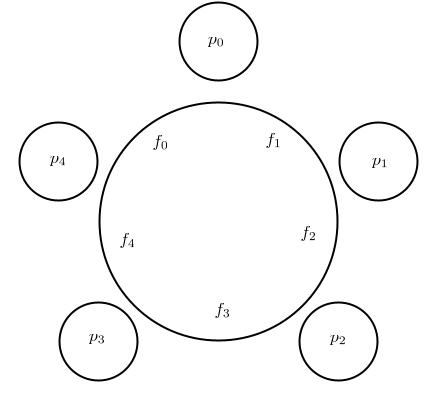
\includegraphics[scale = 0.5]{img/pt10.jpg}
%   \caption{Rappresentazione schematica del problema dei 5 filosofi}
% \end{figure}
% Ogni filosofo ha lo stesso comportamento, un po' pensa e un po' mangia,
% prendendo prima la forchetta alla sua destra e poi quella alla sua sinistra
% (perché necessitano di due forchette per mangiare). Si ha quindi il
% \textit{deadlock} se tutti vogliono mangiare, prendendo tutti in primis una
% forchetta, impedendosi tutti a vicenda di mangiare (non potendo prendere due
% forchette) o si ha la \textit{starvation} in quanto potrebbero accordarsi per
% mangiare in quattro, impedendo a uno di mangiare.\\
% Si vuole modellare tale schema. Ogni filosofo può essere modellato come una rete
% elementare, che farà da componente al modello finale:
% \begin{figure}[H]
%   \centering
%   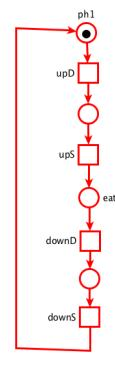
\includegraphics[scale = 0.5]{img/pt11.jpg}
% \end{figure}
% con gli eventi \textit{upD} e \textit{upS}, dove il filosofo prende la forchetta
% destra e sinistra, e rispettivamente \textit{downD} e \textit{downS}, dove le
% mette giù. Si ha la condizione che specifica che il filosofo sta pensando e
% quella che mi segnala l'azione del mangiare, oltre alle due condizioni
% intermedie che separano le azioni tra forchetta sinistra e destra.\\
% Si modella anche la componente della forchetta, con gli eventi che segnalano se
% è depositata, \textit{down}, o meno, \textit{up}:
% \begin{figure}[H]
%   \centering
%   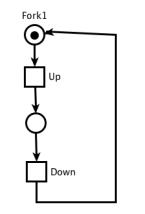
\includegraphics[scale = 0.5]{img/pt12.jpg}
% \end{figure}
% \newpage
% Combino quindi le due componenti per specificare il filosofo che prende la sua
% forchetta destra e poi la sinistra, quindi per ogni componente \textit{filosofo}
% si hanno due componenti \textit{forchetta}:
% \begin{figure}[H]
%   \centering
%   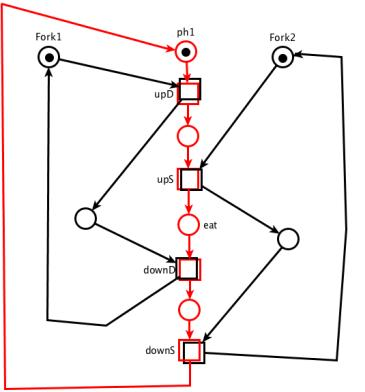
\includegraphics[scale = 0.5]{img/pt13.jpg}
% \end{figure}
% con la \textit{forchetta 1 (fork 1)} che sarà la forchetta destra e la
% \textit{forchetta 2 (fork 2)} che sarà la forchetta sinistra. Si hanno quindi
% diverse transizioni di sincronizzazione tra le due componenti (ogni volta che il
% filosofo interagisce con la forchetta).\\
% Bisogna aggiungere che ogni forchetta può essere presa da due filosofi, ognuna a
% destra di un filosofo e a sinistra di un altro:
% \begin{figure}[H]
%   \centering
%   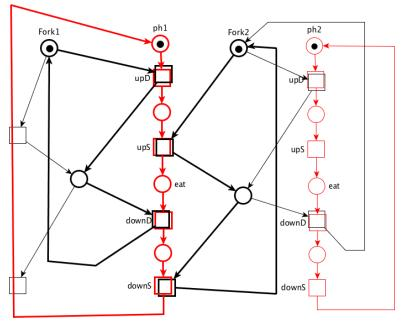
\includegraphics[scale = 0.5]{img/pt14.jpg}
% \end{figure}
% Ogni forchetta quindi si sincronizza alternativamente tra due filosofi, venendo
% presa da uno dei due filosofi. Si è arrivati quindi ad una \textbf{situazione di
%   conflitto}, o meglio ad una \textbf{situazione di confusione}.\\
% Per ora la soluzione di questo problema viene lasciato da parte per valutare il
% modello dello stesso.\\
% Si ha quindi una possibile rappresentazione del modello completo:
% \begin{figure}[H]
%   \centering
%   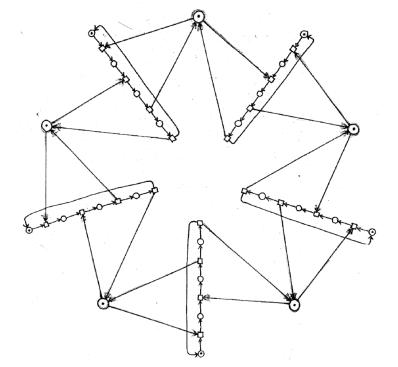
\includegraphics[scale = 0.5]{img/pt15.jpg}
% \end{figure}
% Ma ogni filosofo, come del resto ogni forchetta, si comporta nella stessa
% maniera. Si tenda quindi di \textit{ripiegare} il modello, modellando un
% un'unica componente filosofo con 5 marche distribuite nei vari stati locali del
% filosofo. Stesso discorso per le forchette. Ottengo quindi il seguente modello:
% \begin{figure}[H]
%   \centering
%   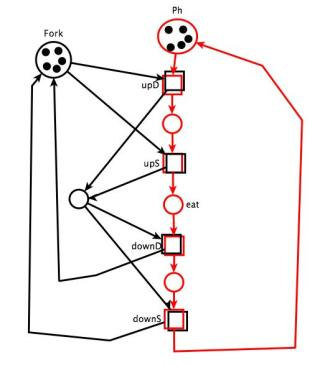
\includegraphics[scale = 0.6]{img/pt16.jpg}
% \end{figure}
% Con le due componenti, \textit{filosofo} e \textit{forchetta}, entrambe
% inizializzate con 5 marche ciascuno. Questo modello però perde informazione
% sulla forchetta che un filosofo può prendere, si ha un radicale \textbf{cambio
%   di protocollo}. Un filosofo può prendere una qualsiasi forchetta e non più
% quella alla sua destra/sinistra. Non possiamo quindi usare le \textit{reti Posti e
%   Transizioni} in quanto perdo troppe informazioni.\\
% L'unica soluzione possibile è quindi quella di recuperare le informazioni perse
% inserendole nelle marche, alle quali viene aggiunta una struttura dati. Si ha
% così modo di distinguere i vari filosofi e le forchette. Per compattare il
% sistema devo quindi rendere più complessa l'essenza della marca, viene
% arricchita con una struttura dati.\\
% Si arriva così ad avere una \textbf{Rete di Alto Livello}, come, per esempio,
% una \textit{rete colorata}, a partire da un rete elementare.\\
% Distinguo quindi filosofi e forchette nei due insiemi di strutture dati:
% \begin{enumerate}
%   \item $Phil=\{p_0,\ldots, p_4\}$, insieme dei filosofi
%   \item $Fork=\{f_0,\ldots, f_4\}$, insieme delle forchette
% \end{enumerate}
% Si nota che per gli indici si ha una somma \textit{modulo 5}, ovvero gli indici
% rispondono alla regola:
% \[(i+1) \mbox{ mod } 5\]
% In modo che gli indici siano ordinati avendo inoltre lo 0 che segue il 4, in
% modo circolare.\\
% Si ottiene quindi, mantenendo il protocollo iniziale:
% \begin{figure}[H]
%   \centering
%   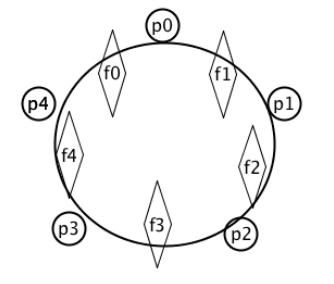
\includegraphics[scale = 0.6]{img/pt17.jpg}
% \end{figure}
% Si mantiene quindi un modello simile a quello descritto sopra ma al posto di
% marche non strutturate si ha nel posto delle 5 forchette le marche dell'insieme
% \textit{Fork} e al posto dei 5 filosofi le marche dell'insieme \textit{Phil}:
% \begin{figure}[H]
%   \centering
%   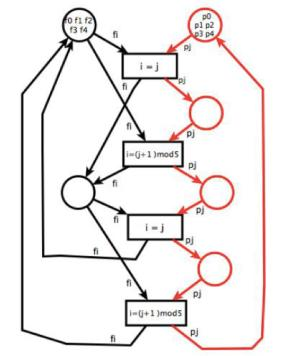
\includegraphics[scale = 0.6]{img/pt18.jpg}
% \end{figure}
% Le transizioni scattano in determinate condizioni. Per esempio la prima
% evento, relativa al fatto che il filosofo prende la forchetta alla sua
% destra, scatta sse con l'istanza filosofo $p_j$ e forchetta $f_i$ si ha che
% $i=j$ (ho quindi almeno una forchetta, almeno un filosofo e la forchetta deve
% essere quella alla sua destra, che, per come abbiamo modellato il problema, è
% quella con lo stesso indice). Sugli archi si hanno quindi annotate determinate
% variabili che denotano istanze. Per la forchetta a sinistra si usa il modulo
% 5. Si procede quindi per i vari filosofi.
% \begin{figure}[H]
%   \centering
%   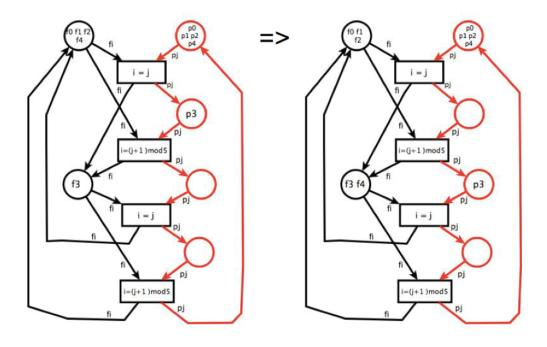
\includegraphics[scale = 0.5]{img/pt19.jpg}
%   \caption{Esempio con il filosofo $p_3$ che ha già preso la forchetta alla sua
%     destra, $f_3$, e prende quella a sinistra, $f_4$}
% \end{figure}
% \textit{Si ha quindi un prezzo per rappresentare in maniera compatta un sistema
%   elementare, mediante una rete di alto livello, ovvero l'arricchimento della
%   struttura dati}.
% \subsection{Formalizzazione delle Reti Posti e Transizioni}
% Nonostante la sezione si occupi di formalismi ci appoggiamo ad un esempio per
% avere un confronto diretto tra teoria e pratica. Questo esempio è un'n-sima
% versione del sistema produttore-consumatore, con un produttore che deposita
% a due elementi alla volta, in un buffer che ha capacità massima apri a cinque,
% che vengono consumati da due consumatori:
% \begin{figure}[H]
%   \centering
%   \begin{tikzpicture}[node distance=2cm, bend angle=45, auto]
%     \node [place, tokens = 1] (p0) [label=above:\small{P2}] {};
%     \node [transition] (t1) [below right of = p0, label=left:\small{d}] {};
%     \node [transition] (t2) [below left of = p0, label=left:\small{p}] {};
%     \node [place] (p1) [below right of = t2, label=below:\small{P1}] {}; 
%     \node [place, tokens=2] (p3) [right of = t1, label=below:$\mbox{B,
%       capacità=5}$] {}; 
%     \node [transition] (t4) [right of = p3, label=right:\small{e}] {};

%     \node [place, tokens=1] (p2) [above right of = t4, label=above:\small{C1}] {}; 
%     \node [transition] (t3) [below right of = p2, label=right:\small{c}] {};
%     \node [place, tokens = 1] (p4) [below right of = t4, label=below:\small{C2}]
%     {}; 
    
%     \path[-{Latex[width=2mm]}]
%     (p0) edge (t1)
%     (t1) edge (p1)
%     (p1) edge (t2)
%     (t2) edge (p0)
%     (t1) edge node {2} (p3)
%     (p3) edge (t4)
%     (t4) edge (p4)
%     (p4) edge (t3)
%     (t3) edge (p2)
%     (p2) edge (t4)
%     ;
%   \end{tikzpicture}
%   \caption{Modello produttore-consumatore compatto con due consumatori.}
% \end{figure}
% quindi al massimo abbiamo cinque marche nel buffer e 2 in uno degli stati del
% consumatore (in quanto rappresenta due consumatori).\\
% Passiamo ora alla formalizzazione:

% \begin{definizione}
%   Si definisce un \textbf{sistema Posti e Transizioni (\textit{sistema P/T})} la
%   sestupla: 
%   \[\Sigma=(S, T, F, K, W;M_0)\]
%   dove:
%   \begin{itemize}
%     \item $(S, T, F)$ è una rete con:
%     \begin{itemize}
%       \item $"S"$ che rappresenta l'insieme dei posti
%       \item $"T"$ che rappresenta l'insieme delle transizioni
%       \item $"F"$ che rappresenta la relazione di flusso che lega posti e
%       transizioni tramite archi
%     \end{itemize}
%     \item $K:S\to\mathbb{N}^{+}\cup \{\infty\}$ che rappresenta una funzione che
%     ad ogni posto in $"S"$ assegna un valore, che può essere un naturale
%     strettamente positivo o anche infinito (ovvero in quel posto possiamo avere un
%     numero qualsiasi di marche). Il valore zero non è ammesso in quanto
%     implicherebbe che il posto non potrebbe mai essere occupato, rendendo la
%     modellazione di un tale posto inutile. $"K"$ è detta \textbf{funzione
%       capacità dei posti}.
%     \item $W:F\to\mathbb{N}$ che rappresenta una funzione che
%     assegna ad ogni arco un peso mediante un valore naturale che stavolta può
%     essere, oltre che infinito, anche zero. $"W"$ è detta \textbf{funzione peso
%       degli archi}
%     \item $M_0:S\to \mathbb{N}\cup\{\infty\}:\,\forall s\in
%     S\,\,\, M_0(s)\leq K(s)$ che rappresenta la \textbf{marcatura iniziale}
%     del sistema, ovvero una funzione che assegna ad ogni posto un naturale,
%     eventualmente nullo o infinito, minore o uguale alla capacità massima di
%     tale posto (capacità espressa dalla funzione $"K"$) indicante il numero di
%     marche allo stato iniziale. 
%   \end{itemize}
%   Bisogna ora definire la regola di scatto, ovvero il \textbf{gioco delle
%     marche}, la regola per cui le marche si spostano sulla rete. Si ha quindi,
%   dati:
%   \[M:S\to\mathbb{N}\cup \{\infty\}\mbox{ e }t\in T\]
%   ovvero data una marcatura e una qualsiasi evento $"t"$ si ha che:
%   \[M[t>\]
%   ovvero una evento è abilitata in una certa marcatura,
%   \begin{center}
%     sse:
%   \end{center}
%   \[\forall s\in S,\,\, M(s)\geq W(s, t)\wedge M(s)+W(t, s)\leq K(s)\]
%   ovvero per ogni posto si ha che ci sono abbastanza marche nei posti perché
%   possa scattare la evento, ovvero c'è un arco di peso corretto che collega
%   quel posto con la evento, avendo peso dell'arco minore o uguale al numero
%   di marche del posto, e, inoltre, si deve verificare che la evento non
%   metta troppe marche in quel posto, quindi la marcatura del posto (ovvero il
%   numero di marche già presenti in esso) più il numero di marche che si
%   aggiungono con lo scatto dell'evento non deve superare la capacità del
%   posto.
%   \begin{figure}[H]
%     \centering
%     \begin{tikzpicture}[node distance=2cm, bend angle=45, auto]
%       \node [transition] (t0) [label=left:$t_3$] {};
%       \node [transition] (t1) [left of = t0, label=left:$t_1$] {};
%       \node [transition] (t2) [right of = t0, label=right:$t_2$] {};
%       \node [place, tokens=2] (p1) [above of = t0, label=above:\small{P1}] {}; 
%       \node [place] (p2) [below of = t0, label=below:$\mbox{capacità=3}$] {}; 
      
%       \path[-{Latex[width=2mm]}]
%       (p1) edge (t1)
%       (p1) edge node {2}(t2)
%       (t1) edge (p2)
%       (t2) edge node {2}(p2)
%       (p2) edge node {3}(t0)
%       (t0) edge (p1)
%       ;
%     \end{tikzpicture}
%     %\includegraphics[scale = 0.75]{img/pt21.jpg}
%     \caption{Nell'esempio si ha che la evento $t_2$ può scattare sse nella
%       posto precedente abbiamo almeno due marche, in quanto l'arco tra i due ha peso
%       due. Inoltre abbiamo il posto che segue vuoto ma con capacità massima pari a
%       tre, quindi la evento può scattare in quanto l'arco tra i due pesa
%       due, assicurandomi che dopo la evento, nel posto che la segue, non
%       verrà superata la capienza massima, arrivando infatti ad avere marcatura
%       pari a 2}
%   \end{figure}
%   Lo scatto dell'evento, se questa è abilitata nella marcatura, mi genera
%   una nuova marcatura che viene ottenuta da quella precedente togliendo tante
%   marche dal posto che è di input alla evento quanto il peso dell'arco che
%   connette tale posto alla evento e aggiungendo tante marche al posto in
%   output quante il peso dell'arco che connette la evento a tale posto,
%   ovvero, formalmente: 
%   \[M[t>M'\]
%   \begin{center}
%     sse
%   \end{center}
%   \[M[t> \wedge\, \forall s\in S,\,\, M'(s)=M(s)-W(s, t)+W(t, s)\]
%   quindi il nuovo posto avrà marcatura pari a quella precedente al più dei due
%   contributi, il primo negativo e il secondo positivo, dei pesi dei due archi.
% \end{definizione} \vspace{5mm} %5mm vertical space
% \begin{definizione}
%   Dato un sistema P/T $\Sigma=(S, T , F , K , W;M_0)$ si definisce
%   l'\textbf{insieme delle marcature raggiungibili}, dalla marcatura iniziale  di
%   $\Sigma$ come:
%   \[[M_0>\]
%   ed esso è il più piccolo insieme tale che:
%   \begin{itemize}
%     \item $M_0\in [M_0>$, ovvero ola marcatura iniziale appartiene all'insieme
%     delle marcature raggiungibili
%     \item se $M\in [M_0> \wedge\,\exists t\in T:\, M[t>M'$ allora $M'\in [M_0$,
%     ovvero se $"M"$ appartiene all'insieme delle marcature raggiungibili ed esiste
%     una evento una evento tale per cui $"M"$ va in $M'$ allora, di
%     conseguenza si ha che $M'$ appartiene all'insieme delle marcature
%     raggiungibili dallo stato iniziale
%   \end{itemize}
%   \emph{Anche questa è una definizione per induzione}

% \end{definizione} \vspace{5mm} %5mm vertical space